%------------------------------------------------------------------------------------------------------
\documentclass[%
%  draft,							% Anschalten f�r Entwurfsstadium
   fontsize=12pt,					% Schriftgroesse der Grundschrift
   paper=a4,						% Papierformat
%  DIV14,							% andere Seitengr��e (siehe Koma Skript Dokumentation !)
   pagesize,						% Schreibt die Papiergroesse in die Datei.
   oneside,							% Einseitiges Layout
   headsepline,					% Linie unter Kolumnentitel ()
   toc=bibliographynumbered,	% Bibliographie ins TOC
%  liststotoc,						% List of figures ins TOC
   numbers=noenddot,				% �berschriftnummerierung ohne Punkt, siehe DUDEN !
   pdftex,							% pdftex Compilierung nutzen
%  fleqn,							% Formeln werden linksbuendig angezeigt
%   showkeys
]{scrbook}
%
%-------------------------Symbole, Schriften etc.------------------------------------------------------
\usepackage[T1]{fontenc}													% Umlaute direkt als ��� eingeben etc.
\usepackage[latin1]{inputenc}											% Latin1-Encodierung (klappt bei mir alles dann)
\usepackage{framed}
\usepackage{xcolor}															% Farben
\usepackage{latexsym,gensymb,textcomp,lmodern,setspace,url}		% Einige Symbole, Schriften etc.
\usepackage[ngerman]{babel}												% Englisches Sprachpaket
%\usepackage{biblatex}
\usepackage{setspace}                                 				% n�tig f�r 1.5- oder 2-fachen Zeilenabstand
\usepackage[section]{placeins}
\onehalfspacing					                          			% anderthalbfacher Zeilenabstand
%
%-------------------------ToDo kennzeichnen------------------------------------------------------------
\newcommand{\workTodo}[1]{\textcolor{red}{todo: #1}}						% Todo-Kennzeichnung
\newcommand{\workMarkDateTime}{\workTodo{\today{} - \thistime\ Uhr}}	% schreibt aktuelle Zeit in die Fu�zeile, damit ihr in der pdf seht, welche Version es ist
%
% Alle Namen hier werden im Titel und im pdf hinterher (hyperref-Paket) eingetragen;
% �berall f�r <Wert> das Entsprechende eintragen und dann das \workTodo entfernen
\newcommand{\workTyp}{Masterarbeit\xspace}
 % <Titel> der Arbeit
\newcommand{\workTitel}{Eine graphische Benutzeroberfl\"ache f\"ur hochdimensionale Quantendynamiksimulationen}
 % <Studiengang> z.B. Kommunikationstechnik
\newcommand{\workStudiengang}{Master Chemie\xspace}
% <Semester> mit Jahr z.B. Sommersemester 2008
\newcommand{\workSemester}{Sommersemester 2014\xspace}
% <Name> des Studenten
\newcommand{\workNameStudent}{Peter Protassow\xspace}
% <Pruefer> Name des pr�fenden (betreuenden) Professor an der Hochschule
\newcommand{\workPruefer}{Prof. Dr.\,Uwe Manthe\xspace}
% <Datum> der Abgabe der Arbeit
\newcommand{\workDatum}{18.\,Juni 2018 \xspace}
% <Betreuer>
\newcommand{\workZweitPruefer}{Prof. Dr.\,Wolfgang Eisfeld\xspace}
% <Zeitraum>
\newcommand{\workZeitraum}{29.\,November 2017 bis 18.\,Juni 2018\xspace}
%
%-------------------------Chemie und Mathe-------------------------------------------------------------
\usepackage{amsmath,amsfonts,amssymb, upgreek,			% verbesserte Matheumgebung und Symbole
bpchem,																% chemische Nomenklatur (Trennung etc.)
chemarrow}															% Darstellung komplexer Reaktionspfeile
\usepackage[fixamsmath,disallowspaces]{mathtools}		% Fehlerbehebung in amsmath
\usepackage{nccmath}
%\usepackage{breqn}
\usepackage{braket}
%\usepackage[version=4]{mhchem}
%multi-part-units=brackets,										% (5\pm 3) kg statt 5 kg \pm 3 kg
%exponent-product=\cdot,											% Schreibweise f�r 5,3*10^3
%group-separator = {,},											% Schreibweise 123,145,175 f�r gro�e Zahlen
%sticky-per,															% \per gilt f�r alle folgenden Einheiten
%separate-uncertainty											% Fehler abtrennen --> 3\pm 1 statt 3(1) im output
%]{siunitx}															% Werte und Einheiten richtig darstellen
%\usepackage[version=3,
%arrows=pgf-filled
%]{mhchem}		% Vereinfachte Schreibweise: \ce{H2O} oder \ce{SO4^{2-}}
%------------------------Tabellen, Grafiken, Zitate und Verweise---------------------------------------
\usepackage{booktabs,multirow,multicol,longtable}		% l�ngere Tabellen m�glich, zusammenh�ngende Zellen
\usepackage[super,square,comma,sort&compress]{natbib}	% Zitationsart angepasst auf Angewandte
%\usepackage{mciteplus}											% verkn�pfte Zitationen

\usepackage{subcaption}
\usepackage{graphicx}											% Grafikunterst�tzung
\usepackage[figurewithin=section]{caption}				% Bildunterschriften
\usepackage{lscape} 											% Tabellen im Querformat m�glich
\usepackage{placeins}

%----------------------Kopf und Fu�zeilen--------------------------------------------------------------
\usepackage{scrpage2}											% Anpassung der Kopf- und Fu�zeilen
\usepackage{scrtime}												% Zeit
\pagestyle{scrheadings}											% Seite mit Headern
\clearscrheadings													% l�scht voreingestellte Stile
\clearscrplain														% l�scht voreingestellte Stile
\chead[]{\leftmark} 											% links: Kapitel (allg. Syntax \Position[scrplain]{scrheadings}; Position: in,out,center,head,foot
\ohead[]{}
\ifoot[\workMarkDateTime]{\workMarkDateTime}				% !!DIESE ZEILE VOR FERTIGSTELLUNG AUSKOMMENTIEREN!!
\ofoot[\pagemark]{\pagemark}									% Seitenzahl
\automark[section]{chapter}                                                      % Inhalt von [\rightmark]{\leftmark}
\setheadsepline{.4pt}[\color{black}]                                             % Linie zwischen Kopf und Textk�rper
%
%--------------------------------------PDF-Links-------------------------------------------------------
\usepackage[pdftex]{hyperref}
\hypersetup{
          pdfhighlight = /O,									% Visualisierung beim Anklicken von Links
   colorlinks=true,												% Links erhalten Farben statt K�stchen
%  urlcolor=black,											% \href{...}{...} external (URL)
%  linkcolor=black,											% \ref{...} and \pageref{...}
%  citecolor=black,											% Literaturverzeichnis
%   urlcolor=darkblue,											% \href{...}{...} external (URL)
   linkcolor=darkblue,											% \ref{...} and \pageref{...}
   citecolor=darkblue,											% Literaturverzeichnis
   % Links
   raiselinks=true,												% calculate real height of the link
   breaklinks,														% Links bestehen bei Zeilenumbruch
   linktocpage=true,												% Inhaltsverzeichnis verlinkt Seiten
   % Bookmarks
   bookmarksopenlevel=1,										% Gliederungstiefe der Bookmarks
   bookmarksopen=true,											% Expandierte Untermenues in Bookmarks
   bookmarksnumbered=true,										% Nummerierung der Bookmarks
   bookmarkstype=toc,											% Art der Verzeichnisses
   plainpages=false,
   pageanchor=true,												% Pages are linkable
   % PDF Informationen
   pdftitle={\workTitel},										% Titel
   pdfauthor={\workNameStudent},										% Autor
   pdfcreator={LaTeX, hyperref, KOMA-Script},			% Ersteller
   pdfstartview=FitB,											% Dokument wird Fit Width ge�ffnet
   pdfpagemode=UseOutlines,									% Bookmarks im Viewer anzeigen
}
\definecolor{green}{rgb}{0,0.5,0}							% gr�n
\definecolor{brown}{rgb}{0.6,0,0}							% braun
\definecolor{darkblue}{rgb}{0,0,.5}							% dunkelblau
\definecolor{lightblue}{rgb}{0.8,0.85,1}					% hellblau
%
%-------------------------Benutzerdefinierte Befehle---------------------------------------------------
\usepackage[ngerman]{varioref}								% Verweise mit automatischer Seitenangabe (\vref{})
\newcommand{\reff}[1]{Abbildung~\ref{#1}\xspace} 		% Verweis auf Abbildung
\newcommand{\reft}[1]{Tabelle~\ref{#1}\xspace}			% Verweis auf Tabelle
\newcommand{\refe}[1]{Gleichung~\eqref{#1}\xspace}		% Verweis auf Gleichung
\newcommand{\ai}{\emph{ab initio}\xspace}
%\renewcommand{\vec}[1]{\underline{#1}}
%\def\Bra#1{\left\langle#1\right|}
%\def\Ket#1{\left|#1\right\rangle}

%\newcommand{\Bra}[1]{\ensuremath{\left\bra #1\right|}}
%\newcommand{\Ket}[1]{\ensuremath{\left| #1\right\ket}}

%\newcommand{\Braket}[2]{\left\langle #1 \middle| #2\right\rangle}
%{\catcode`\|=\active \gdef|{\egroup\,\vrule\,\bgroup}}
%Der vertikale Strich ist aktiv, also
%  \Braket{g|e}
%  \Braket{g|H|e}
\def\sgn{\mbox{\rm sgn}\,}

\newcommand{\diff}{{\rm d}}
\newcommand{\dx}[1]{{\diff}{#1}}
\newcommand{\dd}[2]{\ensuremath{\frac{{\rm d}#1}{{\rm d}#2}}}
\newcommand{\pp}[2]{\ensuremath{\frac{{\partial}#1}{{\partial}#2}}}
\newcommand{\eup}[1]{{\rm e}^{#1}}

\newcommand{\op}[1]{\widehat{#1}}
\newcommand{\hop}{\widehat{H}}

%Erwartungswert:
\newcommand{\ew}[2]{\ensuremath{\left\langle #2\left|#1\right|#2\right\rangle}}
%Skalarprodukt:
%\newcommand{\ip}[2]{\ensuremath{\left\bra #1\left|\right#2\right\ket}}
\newcommand{\ip}[2]{\ensuremath{\left\langle #1 | #2 \right\rangle}}
%Matrixelement:
%\newcommand{\me}[3]{\ensuremath{\left\bra #1\left|#2\right|#3\right\ket}}
\newcommand{\me}[3]{\ensuremath{\left\langle #1 \middle| #2 \middle| #3\right\rangle}}
%
\newcommand{\cv}{C$_{2\text{v}}$}
%C2V Symmetrie
\newcommand{\cm}{cm$^{-1}$}
%inverse Zentimeter
\newcommand{\conf}[4]{$\sigma_b^{#1}\pi_b^{#2}\pi_a^{#3}\sigma_a^{#4}$}
%electronic configuration
\graphicspath{{./figures/}}
%
\begin{document}
\frontmatter
\pagenumbering{Roman}
    %%%%%%%%%%%%%%%%%%%%%%%%%%%%%%%
% R�ckseite Deckblatt

\thispagestyle{empty}
\cleardoublepage
%%%%%%%%%%%%%%%%%%%%%%%%%%%%%%%
% Erste Seite (Titelblatt)

\thispagestyle{empty}
\begin{center}

%    
\includegraphics[width=3cm]{Uni-Logo}\\
%    \vspace{.5cm}
    {\Large Universit"at Bielefeld}\\


    \vspace{.5cm}

    {\huge Fakult"at f"ur Chemie\\[1mm]}


    \vspace{1cm}

    {\Large \textbf{\workTyp}}\\
    \vspace{1.5cm}

    {\huge \textbf{{Eine graphische Benutzeroberfl"ache f"ur hochdimensionale Quantendynamiksimulationen}}}

    % bei k�rzeren Titeln ggf. Schriftgr��e herauf setzen und ein- oder zwei Zeilen streichen

    \vspace*{3mm}
    {\huge \textbf{ }}\\
    \vspace*{3mm}
    {\huge \textbf{}}\\\vspace*{2cm}

    \parbox{1cm}{
      \begin{large}
        \begin{tabbing}
          Bearbeiter: \hspace{1.5cm}
            \=\workNameStudent\\[2mm]
    Pr"ufer: \>\workPruefer\\[2mm]
    Zweitpr"ufer: \>\workZweitPruefer\\[5mm]
    Abgabedatum: \> \workDatum \\
        \end{tabbing}
      \end{large}
    }\\

    \vspace{.3cm}

    
\includegraphics[width=3cm]{Uni-Logo}

\end{center}

    \thispagestyle{empty}
    \cleardoublepage
    \begin{large}

\vspace*{2cm}
\noindent
Hiermit versichere ich, die vorgelegte \workTyp selbstst"andig und ohne unzul"assige Hilfe angefertigt zu haben. Die verwendeten Quellen und Hilfstexte sind vollst"andig angegeben und die Stellen der Arbeit, einschlie"slich Tabellen und Abbildungen, die anderen Werken im Sinn und Wortlaut entnommen wurden, als Entlehnung kenntlich gemacht. Die Bestimmungen der Bachelorpr"ufungsordnung sind mir bekannt. Die von mir vorgelegte \workTyp wurde in der Zeit vom \workZeitraum im Arbeitskreis von Prof. Dr. Uwe Manthe an der Fakult"at f"ur Chemie der Universit"at Bielefeld unter der wissenschaftlichen Anleitung von Roman Ellerbrock durchgef"uhrt.

\vspace{2cm}

\noindent
Bielefeld, den \workDatum .

\vspace{3cm}

\hspace*{7cm}
\dotfill\\
\hspace*{8.5cm}
\textit{(\workNameStudent)}

\end{large}

    \thispagestyle{empty}
    \cleardoublepage
%    \chapter{Danksagung}
Danken m\"ochte ich Prof. Dr. Uwe Manthe f\"ur dieses spannende Projekt.
Ich bedanke mich insbesondere bei meinem Betreuer Roman Ellerbrock, ohne dessen Hilfe und Vertrauen 
diese Arbeit nicht entstanden w"are. 
Au"serdem m"ochte ich mich auch bei der gesamten Arbeitsgruppe der theoretischen Chemie f\"ur die sehr angenehme Arbeitsatmosph\"are bedanken.

    \thispagestyle{empty}
    \tableofcontents
 %   \thispagestyle{plain}
%    \chapter{List of abbreviations}
\begin{tabbing}
\textbf{SO} \qquad \qquad \qquad \=-- spin-orbit\\



\textbf{CI}		\>-- configuration interaction\\
\textbf{MRCI}		\>-- multiconfiguration reference singles and doubles configuration interaction\\
\textbf{CASSCF}		\>-- complete active space self-consistent field\\
\textbf{AO} 		\>-- atomic orbital\\
\textbf{MO} 		\>-- molecular orbital\\
\textbf{ECP}		\>-- effective core potential\\
\textbf{RECP}		\>-- relativistic effective core potential\\
\textbf{aug-cc-pVTZ}	\>-- augmented correlation consistent polarized valence triple $\zeta$ basis set\\
\textbf{MRQDPT2}	\>-- multi-reference quasi-degenerate second-order pertubation theory \\
\textbf{EOM-CCSD}	\>-- scalar equation of motion coupled cluster \\
\textbf{MR-CIS}		\>-- multi-reference configuration interaction with single excitations \\ 


\textbf{ERCAR}		\>-- effective relativistic coupling by asymptotic representation\\

\end{tabbing}


% ---------------------------------------------------------------
\mainmatter
     \chapter{Einleitung}

In der Physik und theoretischen Chemie hat sich die multiconfigurational time-dependent Hartree (MCTDH)-Methode
als effizienter Algorithmus zur L"osung der zeitabh"angige Schr"odingergleichung etabliert.
Um mit der MCTDH-Methode arbeiten zu k"onnen, sind bisher fortgeschrittene Programmierkenntnissen Voraussetzung.\\
Um das Arbeiten mit der MCTDH-Methode auch anderen Wissenschaftlern mit wenig Programmiererfahrung zu erm"oglichen,
soll in dieser Arbeit eine grafische Oberfl"ache (GUI) implementiert werden.
Es wurde existierender MCTDH-C++ Code gewrappt. Der gewrappte Code wurde f"ur den Aufbau der GUI verwendet.

     \chapter{MCTDH Theorie}

\section{Einleitung}
Die Entwicklung von Methoden, die eine genaue quantendynamischen Berechnung von mehratomaren Systemen erm"oglichen, stellen die theoretische Chemie und
chemische Physik vor eine wesentliche Herausforderung.
Der MCTDH-Ansatz[16,17paper] spielt eine entscheidende Rolle am Erfolg der Entwicklung quantendynamischer Rechenmethoden.
Mit dem MCTDH-Ansatz konnten Reaktionsraten von Reaktionen mit sechs Atomen wie $H+CH_{4} \rightarrow H_{2} + CH_{3}$ [10-14paper]
und $ O + CH_{4} \rightarrow OH + CH_{3} $ [15paper] berechnet werden.
Des Weiteren konnten Tunnelaufspaltungen und Schwingungszust"ande von Malonaldehyd[18paper] und dem $ H_{5}O^{+}_{2} $-Cluster[7-9paper] berechnet werden.
Sowohl die Schwingungsdynamiken von lichtangeregten Pyrazin [19paper] und von photoionisierten Butatrien [20paper] als auch der Elektronentransfer
aus einem angeregten Zustandes in "Ubergangsmetallen [21,22paper]  konnten mithilfe des MCTDH-Ansatzes untersucht werden.
\\Um molekulare Systeme theoretisch untersuchen zu k"onnen, muss zun"achst die Schr"odingergleichung (SGL) gel"ost werde.
Um die SGL zu l"osen, muss die Wellenfunktion, die das System beschreiben soll, definiert werden.
Generell wird die Wellenfunktion durch das Produkt von mehrdimensionalen zeitabh"angigen Basisfunktionen dargestellt.
Dieser Ansatz der Wellenfunktion wird in der Standardmethode verwendet. [meyer rev 2011]
 Die Basisfunktionen werden in einer eindimensionalen zeitunabh"angigen Basis mit den jeweiligen zeitabh"angigen Koeffizienten entwickelt.
F"ur jeden Freiheitsgrad $f$ des Systems ergeben sich $N$ zeitunabh"angige Basisfunktionen. Somit w"achst die Anzahl der Entwicklungskoeffizienten um $N^{f}$ und
die Standardmethode skaliert exponentielle, sodass nur kleinere Systeme berechenbar sind. [meyer rev 2011]
  \\ Im Unterschied zu der Standardmethode resultiert die Effizienz des MCTDH aus der Doppellayerstruktur der verwendeten Wellenfunktion.
Anstelle die Wellenfunktion in einer zeitunab"angigen Basis zu entwickeln und die Zeitentwicklung durch zeitabh"angige Entwicklungskoeffizienten zu beschreiben,
wird in der MCTDH - Methode die Wellenfunktion als ein Satz von zeitabh"angigen Basisfunktionen dargestellt.
Diese zeitabh"angigen Basisfunktionen werden Einteilchenfunktionen (SPF) genannt und in einer primitiven zeitunabh"angigen Basis dargestellt.
Die Doppellayerstruktur des MCTDHs resultiert aus zwei Entwicklungen mit jeweils zeitabh"angigen Entwicklungskoeffiziente:
Zum einen stellen die Entwicklungskoeffizienten mit den SPFs die korrelierte Wellenfunktion dar und bilden den oberen MCTDH -
Layer und zum anderen k"onnen die SPFs durch die Entwicklungskoeffizienten in der primitiven zeitunabh"angigen Basis entwickelt werden. Diese Entwicklung bildet
den unteren Layer.[Manthe, 2008 multilayer MCTDH approach]
  \\ Die Anzahl der SPFs kann verglichen mit der primitiven Basis signifikant kleiner gew"ahlt werden.
Dennoch ist auch das MCTDH durch eine exponentielle Skalierung limitiert.
Um Korrelationseffekte beschreiben zu k"onnen, sind mindestens zwei SPFs pro Freiheitsgrad notwendig, sodass der numerische Aufwand mit der Anzahl der
Freiheitsgrade $f$ zu $2^f$ skaliert. Aufgrund dieser Skalierung k"onnen Systeme mit maximal 12 - 14 korrelierten Koordinaten [10-15,27,28] behandelt werden.
  \\ Zus"atzliche zu der Doppellayerstruktur k"onnen die Koordinaten in ,,logische`` und physikalische Koordinaten unterschieden werden und
verschiedene physikalischen Koordinaten werden zu einzelne logische Koordinaten kombiniert. Die logischen Koordinaten werden Partikel genannt, sodass
nicht die Anzahl der Freiheitsgrade der limiterende Faktor f"ur die modenkombinierte MCTDH-Rechnung ist,
sondern die Anzahl der Partikel $p$. So konnten Systeme mit 15 - 24 korrelierten Freiheitsgraden [8,9,19,20] und System-Bad-Modelle [31-33] behandelt werden.
Dennoch bleibt das Problem der exponentielle Skalierung von $2^p$ bestehen.
  \\Dieses Problem wird mit dem multilayer (ML)-MCTDH-Ansatz [34] begegnet.
Die SPFs k"onnen selbst als mehrdimensionale Wellenfunktionen dargestellt werden und in anderen SPF entwickelt werden.
Bei drei Layern wird der obere Layer durch die SPF-Basis des herk"ommlichen MCTDHs gebildet.
Diese Basis wird als SPFs des ersten Layers bezeichnet und kann selbst in der SPF-Basis des zweiten Layers entwickelt werden.
Die SPF-Basis des zweiten Layers erweitert das MCTDH um einen weiteren Layer und wird selbst in der primitiven Basis entwickelt, die den unteren Layer bildet.
Durch die rekursive Anwendung der MCTDH - Methode k"onnen weitere Layer zugef"ugt.
Mit der ML-MCTDH Methode sind quantumdynamische Rechnungen von System-Bad Modellen mit bis zu 1000 korrelierten Koordinaten m"oglich,
in denen Elektronentransferprozesse [34-35] untersucht wurden.
 \\Um die MCTDH-Wellenfunktion propagieren zu k"onnen, m"ussen die Matrixelemente des Hamiltonoperators effizient berechnet werden.
So lange der Hamiltonoperator der Summe von Produkten von Einteilchenoperatoren [17] entspricht, stellt die Berechnuung der Matrixelemente kein Probelm dar.
Im Gegensatz zu vielen Modelhamiltonoperatoren k"onnen \textit{ab initio} Potentialenergiefl"achen nicht in dieser Form dargestellt werden.
Durch die Verwendung einer spezifischen zeitabh"angigen Quadratur, die die Matrixelemente allgemeiner Potentiale effizient auswertet, k"onnen
auch Matrixelemente solcher \textit{ab initio} Potentialenergiefl"achen effizient berechnet werden.
Diese Vorgehensweise wird correlation discrete variable representation (CDVR) [40,41] genannt.
 \\Das urspr"ungliche Vorgehen f"ur das CDVR [40] beruht auf ein zeitabh"angiges DVR-Gitter, das direkten Produkten einer SPF-Basisfunktion entspricht.
Somit kann das Standard-CDVR weder f"ur modenkombinierte MCTDH-Rechnungen noch f"ur Berechnungen mit dem ML-MCTDH-Ansatz verwendet werden.
 \\Allerdings konnte ein CDVR , das ohne ein direktes Produktgitter auskommt, in modenkombinierte MCTDH-Rechnungen verwendet werden. [42]
 Der numerische Aufwand des CDVRs h"angt linear von der Anzahl der verwendeten primitiven Gitterpunkten ab, die f"ur die Darstellung der SPFs ben"otigt werden.
In modenkombinierte MCTDH-Rechnungen wird eine gro"se Anzahl an primitiven Gitterpunkten verwendet, sodass modenkombinierte MCTDH-Rechnungen kombiniert mit CDVR-
Auswertung des Potentials ineffizient sind. ML-MCTDH-Rechnungen ben"otigen dagegen keine mehrdimensionalen Gitter, um die SPFs darzustellen, und bieten sich
in Kombination mit dem CDVR an.

\section{Layerstruktur der MCTDH - Wellenfunktion}

Ziel ist es die zeitabh"angige SGL

\begin{equation}
i\dot{\Psi} = H \Psi
\label{Eq:SGL}
\end{equation}

zu l"osen.
  \\Zur L"osung von Gleichung \ref{Eq:SGL} kann die Wellenfunktion $\Psi$ in einer zeitunabh"angigen Basis $\mathcal{X}^{\kappa}_{j}(x_{\kappa})$ entwickelt werden:

 \begin{equation}
 \Psi(x_{1},..., x_{f}, t)=\sum^{N_{1}}_{j_{1}=1} ... \sum^{N_{f}}_{j_{f}=1} A^{1}_{j_{1}, ..., j_{f}}(t)\cdot \mathcal{X}^{(1)}_{j_{1}}(x_{1}) \cdot ... \cdot \mathcal{X}^{(f)}_{j_{f}}(x_{f})
 \label{Eq:Std_wave}
 \end{equation}

Die zeitabh"angigen Koeffizienten $A^{1}_{j_{1}, ..., j_{f}}(t)$ beschreiben die Bewegung der Wellenpakete.
Die Darstellung der Wellenfunktion in Gleichung  \ref{Eq:Std_wave} kann auch als Einfachlayerdarstellung betrachtet werden.
Im Unterschied zu Gleichung \ref{Eq:Std_wave} wird die MCTDH - Wellenfunktion,

 \begin{equation}
 \Psi(x_{1},..., x_{f}, t)=\sum^{n_{1}}_{j_{1}=1} ... \sum^{n_{f}}_{j_{f}=1} A^{1}_{j_{1}, ..., j_{f}}(t)
 \cdot \phi^{1;1}_{j_{1}}(x_{1}, t) \cdot ... \cdot \phi^{1;f}_{j_{f}}(x_{f}, t)
 \label{Eq:mctdh_wave}
 \end{equation}

in der zeitabh"angigen SPF - Basis $\phi^{\kappa}_{j}(x_{\kappa})$ entwickelt, die wiederum in der primitiven Basis $\mathcal{X}^{\kappa}_{j}(x_{\kappa})$ entwickelt wird:

\begin{equation}
 \phi^{1;\kappa}_{m} (x_{\kappa}, t)=\sum^{N_{\kappa}}_{j=1} A^{2;\kappa}_{m;j}(t) \cdot \mathcal{X}^{(\kappa)}_{j}(x_{1})
 \label{Eq:SPF}
 \end{equation}

Die hochgestellte Zahl $z$ der Koeffizienten $A^{z}(t)$ bezieht sich auf die Layertiefen.
In Gleichung \ref{Eq:SPF} folgt aus $z=2$, das Gleichung \ref{Eq:SPF} den zweiten Layer darstellt.
Gleichzeitig ist Gleichung \ref{Eq:SPF} der letzte Layer, da in der primitiven Basis entwickelt wurde.
Das hochgestellte $\kappa$ und der Index $m$ von $A^{2;\kappa}_{m;j}(t)$ beziehen sich auf die $m$-te SPF und die $\kappa$-te Koordinate.
Die Hochzahl $s$ in $ \phi^{s;\kappa}_{m} (x_{\kappa}, t) $ entspricht dem Layer, der durch jeweiligen SPFs representiert wird
und ist durch die maximale Anzahl der Layer begrenzt.
  \\Zur Visualisierung der Layerstruktur des MCTDHs dienen die Diagramme f"ur die unterschiedlichen Darstellungen der Wellenfunktionen in Abbildung \ref{fig:tree}.
Abbildung \ref{fig:std_wave} stellt die Wellenfunktion aus Gleichung \ref{Eq:Std_wave} schematisch dar, wobei alle Wellenfunktionen von Abbildung \ref{fig:std_wave}
bis \ref{fig:multi_mctdh_wave} ein siebendimensionalen System beschreiben.
In den Diagrammen werden die verschiedenen S"atze der A-Koeffizienten durch die ausgef"ullten schwarzen Kreise repr"asentiert.
So kommen in Abbildung \ref{fig:std_wave} nur die Koeffizienten $A^{1}_{j_{1}, ..., j_{7}}$ vor, die durch den
einzigen schwarzen Punkt gekennzeichnet sind.
  \\Im Unterschied zur Wellenfunktion aus \ref{Eq:Std_wave} besitzt die MCTDH-Wellenfunktion
in Abbildung \ref{fig:mctdh_wave} zwei Layer.
Somit beinhaltet die Beschreibung der Wellenfunktion mehrere S"atze an A-Koeffizienten.
Die Koeffizienten $A^{2;\kappa}_{m;j}$ werden durch alle schwarzen Punkte, die horizontal angeordnet und mit den obersten Punkt verbunden sind, dargestellt.
Dabei sind $A^{2;\kappa}_{m;j}$ und $A^{1}_{j_{1}, ..., j_{7}}$ durch Line verbunden, die jeweils den Index $m$ repr"asentieren.
Jede darauffolgende Linie, die die $A^{2;\kappa}_{m;j}$ mit den sieben Koordinaten $x_{1}, x_{2}, ..., x_{7}$ verbindet, entspricht einer der sieben Indizes $j$.
Somit existieren sieben S"atze von A-Koeffizienten $A^{2;1}, A^{2;2}, ..., A^{2;7}$, den zweiten Layer beschreiben.
In Abbildung \ref{fig:std_wave} ist der Koeffizient $A^{1}_{j_{1}, ..., j_{7}}$ direkt mit den Koordinaten verbunden.
  \\Die Koordinaten der modenkombinierte MCTDH-Wellenfunktion werden im Gegensatz zur Doppellayerwellenfunktion \ref{Eq:mctdh_wave}  in $d$ logischen Koordinaten
  eingeteilt, sodass mehrdimensionale SPFs verwendet werden. Die mehrdimensionalen Koordinaten $q^{1}_{1}, q^{1}_{2}, ..., q^{1}_{d}$
  werden wie folgt definiert:


\begin{equation}
%\label{eqn:eqlabel}
\begin{gathered}
   q^{1}_{1} = \{q^{2;1}_{1},q^{2;1}_{2},q^{2;1}_{d_{1}}\} = \{x_{1}, x_{2}, ..., x_{d_1}\} \\
  q^{1}_{2} = \{q^{2;2}_{1},q^{2;2}_{2},q^{2;2}_{d_{2}}\} = \{x_{d_{1}+1}, x_{d_{1}+2}, ..., x_{d_{1}+d_{2}}\} \\
  q^{1}_{d} = \{q^{2;d}_{1},q^{2;d}_{2},q^{2;d}_{d_{d}}\} = \{..., x_{f}\}
\end{gathered}
\end{equation}

Die logische mehrdimensionale Koordinate $ q^1_\kappa $ umfasst $d_\kappa $ Koordinaten, wobei $\kappa$ den Index der Koordinate des ersten Layers angibt
und werden immer mit einer eins als Hochzahl angegeben, da es sich bei den logischen Koordinaten immer um Koordinaten des ersten Layers handelt.
Enthalten in den logischen Koordinaten sind Koordinaten des zweiten Layers : $  q^{2;\kappa}_1, q^{2;\kappa}_2, ..., q^{2;\kappa}_{d_\kappa} $, auf den durch die
zwei als Hochzahl hingewiesen wird. Alle Koordinate des zweiten Layers entsprechen den jeweiligen physikalischen Koordinaten $x_{1}, x_{2}, ...$ und $x_{f}$.
Eine modenkombinierte MCTDH-Wellenfunktion kann dann wie folgt definiert werden:

\begin{equation}
 \Psi(q^{1}_{1},q^{1}_{2},..., q^{1}_{d}, t)=\sum^{n_{1}}_{j_{1}=1} ... \sum^{n_{d}}_{j_{d}=1} A^{1}_{j_{1}, ..., j_{d}}(t)
 \cdot \phi^{1;1}_{j_{1}}(q^1_{1}, t) \cdot ... \cdot \phi^{1;d}_{j_{d}}(q^1_{d}, t)
 \label{Eq:mode_comb_wave}
 \end{equation}

\begin{equation}
  \begin{gathered}
 \phi^{1;\kappa}_{m} (q^1_{\kappa}, t)=\sum^{N_{\alpha}}_{j=1} ... \sum^{N_{\beta}}_{j_{d_\kappa}=1} A^{2;\kappa}_{m;j_1,...,j_{d_\kappa}}(t)
 \cdot \mathcal{X}^{(\alpha)}_{j_1}(q^{2;\kappa}_1) \cdot ... \cdot
 \mathcal{X}^{(\beta)}_{j_{d_\kappa}}(q^{2;\kappa}_{d_\kappa})\\
 \left( \alpha = 1 + \sum^{\kappa - 1}_{i=1}d_i \text{ and }  \beta = 1 + \sum^{\kappa}_{i=1}d_i\right)
 \label{Eq:mode_SPF}
\end{gathered}
 \end{equation}

In Abbildung \ref{fig:mode_wave} sind die sieben physikalischen
Koordinaten in drei mehrdimensionale logische Koordinaten der Wellenfunktion $ \Psi(q^{1}_{1},q^{1}_{2},q^{1}_{3}, t)$ aufgeteilt: $q^{1}_{1} = \left(x_1, x_2 \right)$, $ q^{1}_{2} = \left(x_3, x_4 \right)$
und $ q^{1}_{3} = \left(x_5, x_6, x_7 \right)$.


\begin{figure}
\begin{minipage}{0.45\textwidth}
    \centering
    \captionsetup[subfigure]{position=top, labelfont=bf,textfont=normalfont,singlelinecheck=off,justification=raggedright}
    \begin{subfigure}[a]{\textwidth}
        \caption{}\label{fig:std_wave}
        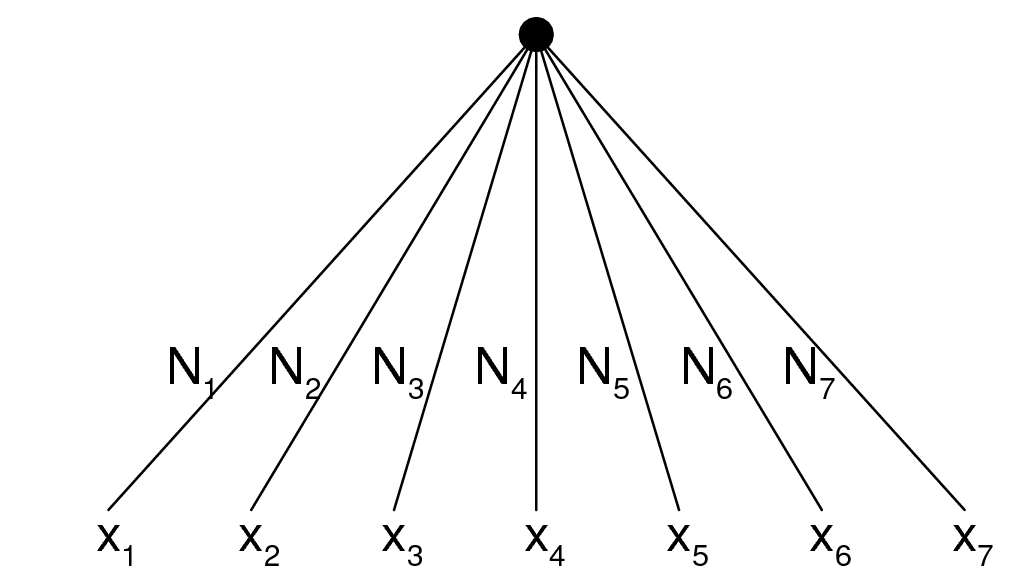
\includegraphics[width=\textwidth]{figures/std_wave}
    \end{subfigure}
    \hfill
    \quad
    \begin{subfigure}[c]{\textwidth}
        \caption{}\label{fig:mctdh_wave}
        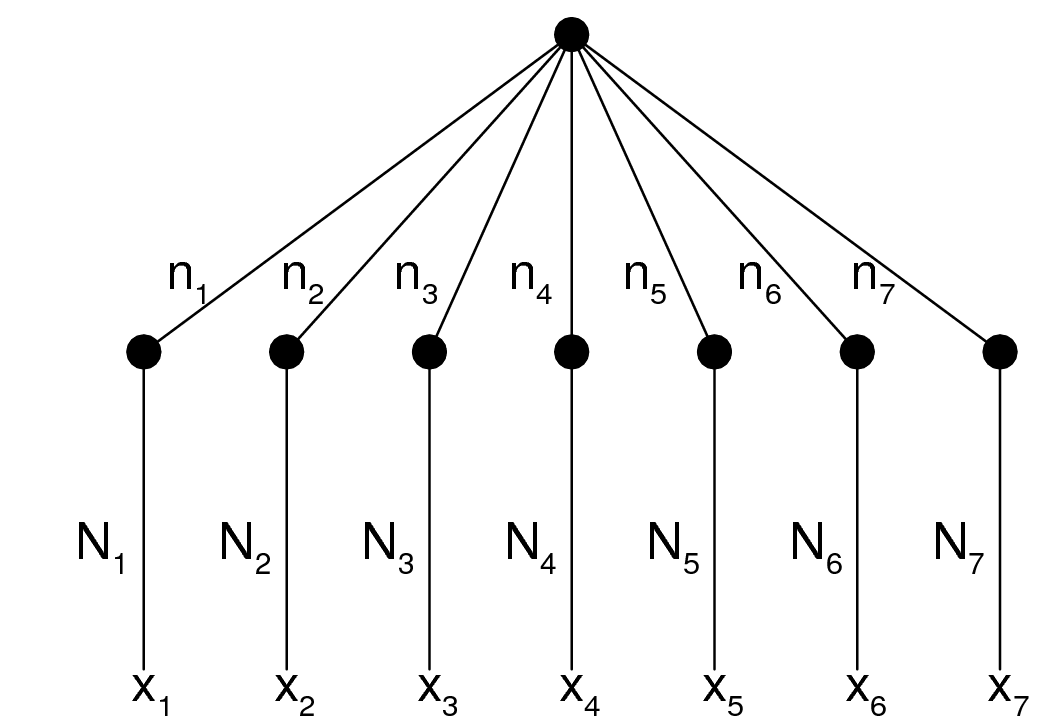
\includegraphics[width=\textwidth]{figures/mctdh_wave1}
    \end{subfigure}
  %  \caption{Left}\label{fig:left}
\end{minipage}
\quad
\begin{minipage}{0.45\textwidth}
    \centering
    \captionsetup[subfigure]{position=top, labelfont=bf,textfont=normalfont,singlelinecheck=off,justification=raggedright}
    \begin{subfigure}{\textwidth}
        \caption{}\label{fig:mode_wave}
        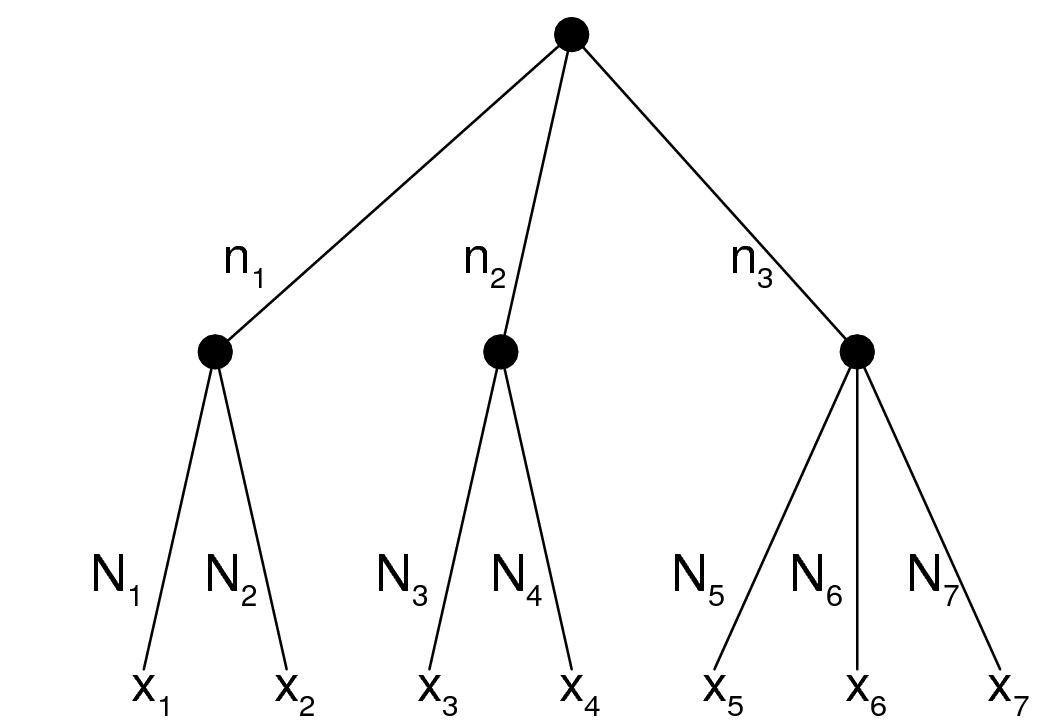
\includegraphics[width=\textwidth]{figures/mctdh_wave2}
    \end{subfigure}
    \quad
    \begin{subfigure}{\textwidth}
        \caption{}\label{fig:multi_mctdh_wave}
        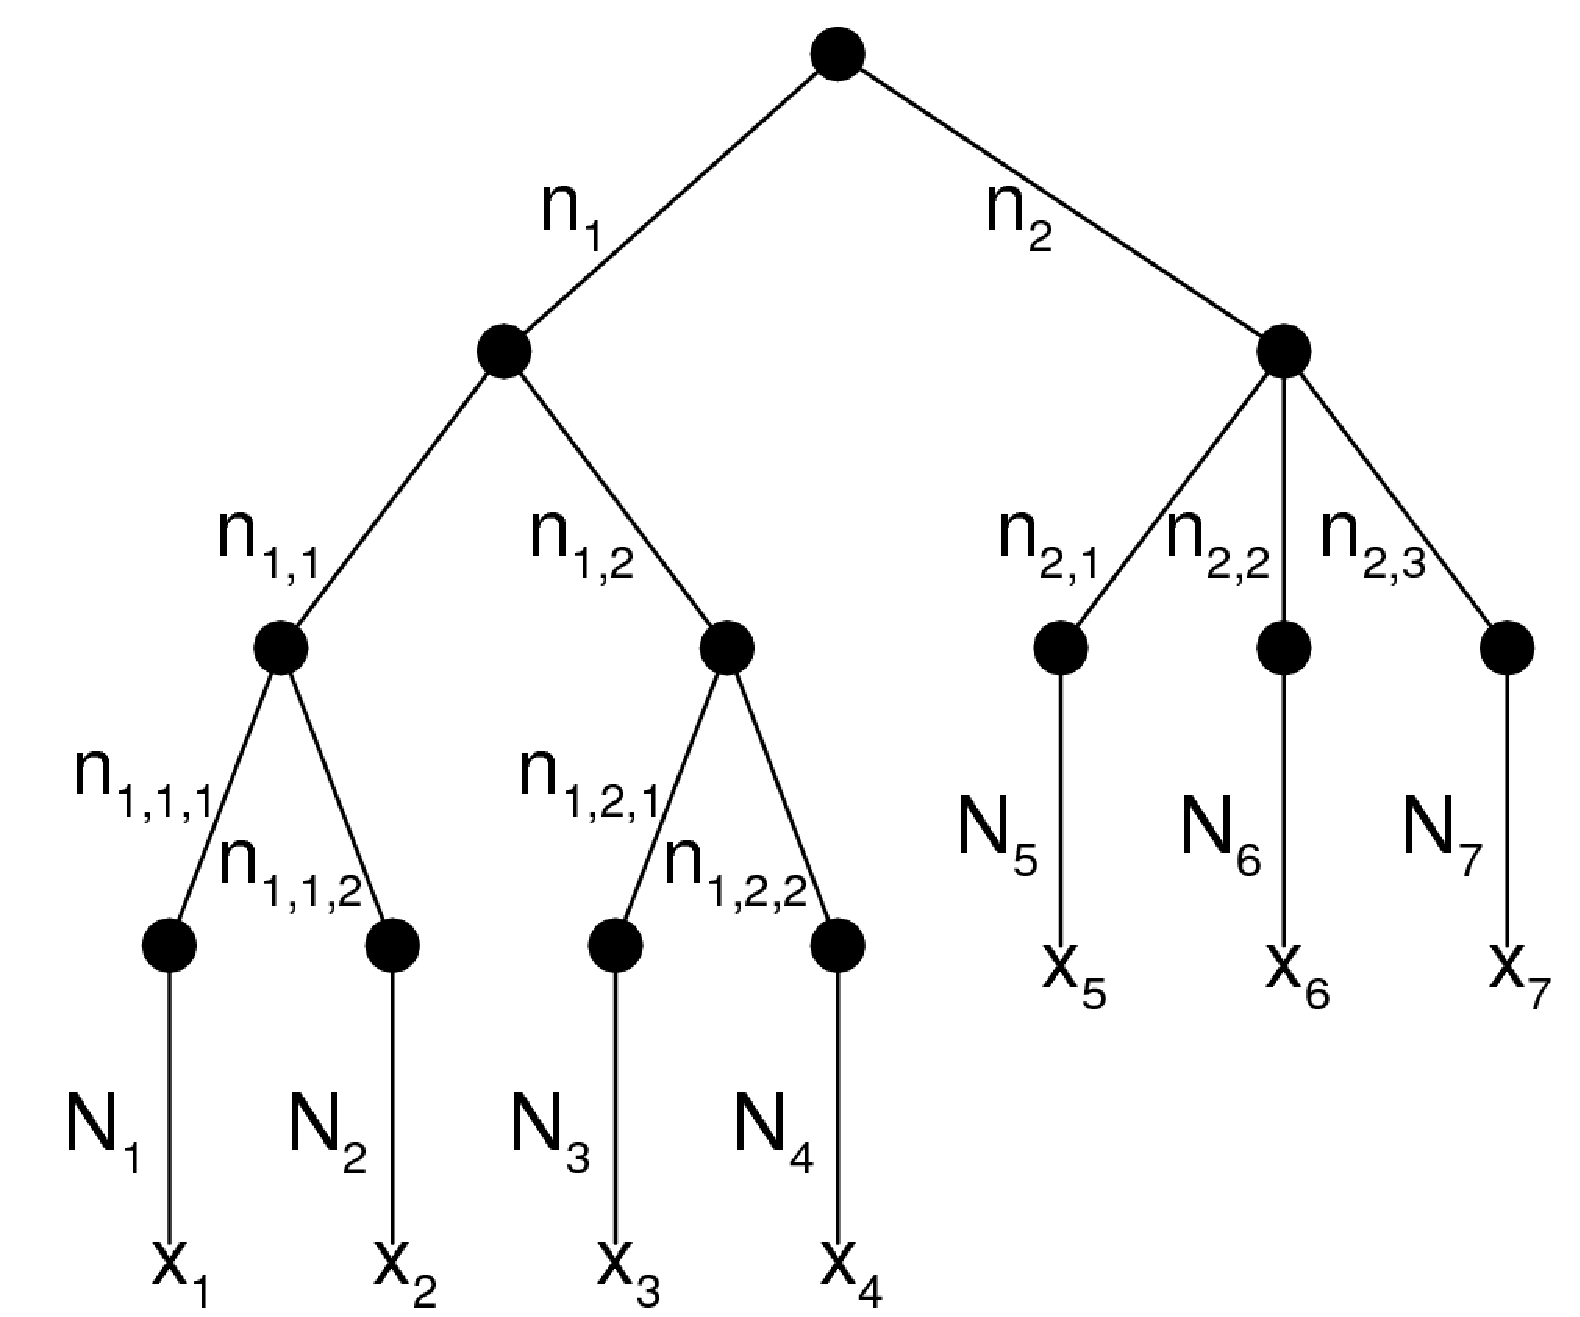
\includegraphics[width=\textwidth]{figures/multi_mctdh_wave}
    \end{subfigure}
%    \caption{right}\label{fig:right}
\end{minipage}
  \caption{Unterschiedliche Darstellung von Wellenfunktionen eines siebendimensionalen Systems. Dargestellt sind: (a) Eine Standard Wellenfunktion,
  (b) eine MCTDH-Wellenfunktion, (c) eine modenkombinierte MCTDH-Wellenfunktion und (d) eine ML-MCTDH-Wellenfunktion.}\label{fig:tree}
\end{figure}

Anstelle die SPFs aus Gleichung \ref{Eq:mode_comb_wave} in einer primitiven Basen zu entwickeln, k"onnen die SPFs des ersten Layers
durch SPFs eines zweiten Layers dargestellt werden. Die SPFs des ersten Layers werden analog zu einer MCTDH-Wellenfunktion entwickelt.
Diese Entwicklung f"uhrt zu einer ML-MCTDH-Wellenfunktion:

\begin{equation}
  \begin{gathered}
 \phi^{1;\kappa}_{m} (q^1_{\kappa}, t)=\sum^{n_{\kappa,1}}_{j=1} ... \sum^{n_{\kappa,d_\kappa}}_{j_{d_\kappa}=1} A^{2;\kappa}_{m;j_1,...,j_{d_\kappa}}(t)
 \times \phi^{2;\kappa,1}_{j_1} (q^{2;\kappa}_{1}, t) \cdot ... \cdot
 \phi^{2;\kappa,d_\kappa}_{j_{d_\kappa}} (q^{2;\kappa}_{d_\kappa}, t)
\\
 \phi^{2;\kappa, \lambda}_{m} (q^{2;\kappa}_{\lambda}, t)= \sum^{N_{\alpha}}_{j=1} A^{3;\kappa, \lambda}_{m;j}(t)
 \mathcal{X}^{(\alpha)}_{j}(q^{2;\kappa}_\lambda)
\\
 \left( \text{ mit } \alpha = \lambda + \sum^{\kappa - 1}_{i=1}d_i \right)
 \label{Eq:ml_mctdh_mode_SPF}
\end{gathered}
 \end{equation}

Die Indizes $\kappa$ und $\lambda$ des SPFs des zweiten Layers $ \phi^{2;\kappa, \lambda}_{m}  $  sind durch die Koordinaten und deren
Zugeh"origkeit zu den logischen Koordinate festgelegt.
Die Koeffizienten $A^{2;\kappa}_{m;j_1,...,j_{d_\kappa}}$ definieren weiterhin die Entwicklung der SPFs des ersten Layers.
Allerdings werden anstelle der zeitunbh"angigen primitiven Basis die zeitabh"angigen SPFs des zweiten Layers als Basis verwendet.
Diese wiederum werden in der primitiven Basis entwickelt und diese Entwicklung wird durch den Koeffzienten  $A^{3;\kappa, \lambda}_{m;j}$
definiert.
  \\Die ML-MCTDH Darstellung kann auf eine beliebige Anzahl von Layern erweitert werden.
  Dabei kann die Anzahl der Layer f"ur die jeweiligen Koordinaten variieren. So werden in Abbildung \ref{fig:multi_mctdh_wave} f"ur die Koordinaten $x_1-x_4$ drei Layer 
  und f"ur die Koordinaten $x_5 - x_7$ zwei Layer verwendet.









\clearpage
 \subsection{Absorption und Emission}

%     \chapter{Technische Details}
\label{cha:Tech}

Die Python-Schnittstelle f"ur MCTDH wurde in der Programmiersprache Cython erstellt. 
Cython stellt eine Hybridprogrammiersprache dar,
die Python und C\textbackslash C++ kombiniert. Im Gegensatz zu Python
wird Cython kompiliert, wobei die Cythonsyntax der Pythonsyntax "ahnlich ist.
In Cython kann C++ Code verwendet werden, der beim Erstellen der Cython-Programme ebenfalls kompiliert wird.
Auf diese Weise wurden mehrere \textit{mctdh}-Klassen auf Basis von C++ Klassen erstellt.

Die GUI f"ur die MCTDH-Rechnungen wurde in Python und Qt implementiert.
Der Zugriff auf die Qt-Bibliothek erfolgt "uber die Python-Bibliothek PyQt4. 
Das Design der einzelnen GUI-Fenster erfolgte in Qt-Designer. Die Informationen "uber 
die jeweiligen Fenster werden in \textit{ui}-Dateien gespeichert. Mit PyQt k"onnen diese Dateien eingelesen werden und die entsprechenden 
Klassen erstellt und beliebig erweitert werden.
Die in Qt-Designer erstellten Fenster werden in PyQt miteinander verkn"upft.

Neben PyQt wurden die Python-Module \textit{networkx} und \textit{matplotlib} verwendet.
Mithilfe von Klassen aus \textit{networkx} und \textit{matplotlib} konnten Baumdiagramme erstellt und gespei\-chert werden, die in der GUI zur 
Visualisierung des MCTDH-Baums verwendet wurden.

  




   

     \chapter{Ergebnisse}

\section{Python-Interface f"ur MCTDH}
\label{sec:PyInterface}


Es wurden eine Programmierschnittstelle (englisch \textit{application programming interface}, API) f"ur das MCTDH-Programmpaket erstellt.
Im Rahmen dieser Arbeit wurde sich auf Klassen beschr"ankt, welche f"ur das Einlesen der baumf"ormig strukturierten MCTDH-Basis zust"andig sind.
Die Klassen und Methoden, die "uber Python aufgerufen werden k"onnen, sind in Abbildung \ref{fig:uml_Cython} dargestellt. 
Jede Klasse der API wird in Abbildung \ref{fig:uml_Cython} durch einen Kasten repr"asentiert. Im oberen Teil des Kastens ist der Klassenname
angegeben und im unteren Teil sind die Methoden der Klasse aufgelistet. Die Anordnung der K"asten gibt die Abh"angigkeit der Klassen zueinander wieder.
So muss er ein Objekte von der Klasse \textit{ControlParameter} initialisiert sein, bevor Methoden der Klasse
\textit{mctdhBasis} verwendet werden k"onnen. Analog h"angen die Klassen \textit{Tdim} und \textit{physCoor} von der Klasse
\textit{mctdhNode} ab.
\textit{ControlParameter} und \textit{mctdhBasis} sind die Klassen, die die Konfigurations- und Basisdatei einlesen. 
In der Klasse \textit{mctdhBasis} kann die Anzahl der Knoten des MCTDH-Baums aus dem Basisdatei ausgegeben werden.
Knoteneigenschaften k"onnen "uber die Klasse \textit{mctdhNode}  ermittelt werden. Dabei stellt ein Objekte dieser Klasse
eine Knoten dar.
So kann festgestellt werden, ob ein Knoten den obersten Knoten darstellt oder zu den untersten Knoten geh"ohrt und mit wieviel weiteren Knoten er verbunden ist.
Die Knotenobjekte k"onnen in Nachbarknoten "uberf"uhrt werden.
Die SPFs eines Knoten wird in der Klasse \textit{Tdim} ermittelt. Mit der Klassen \textit{physCoor} k"onnen
die Schwingungsmoden, der untersten Knoten bestimmt werden. 


Zur Demostration der API wird im folgenden ein Python-Skript vorgestellt, mithilfe dessen die Gr"o"se einer MCTDH-Wellenfunktion berechnet wird:
\newpage
\begin{verbatim}
import mctdh

config = mctdh.controlParameters()
config.initialize(mctdh.config)
basis = mctdh.MctdhBasis()
basis.initialize('basis.txt', config)

maxNodes = basis.NmctdhNodes()

nodes_spf = {}
sumBottomNode = {}
remnantNodeList = []

def get_SPFs():
    SumTopNode = 0
    remnantNode = 0

    for i in range(maxNodes):
        node = basis.MCTDHnode(i)
        tdim = node.t_dim()
        nodes_spf[i] = tdim.GetnTensor() 
    mode_spf = {i: basis.MCTDHnode(i).t_dim().active(0) for i in \
                range(maxNodes) if \
                basis.MCTDHnode(i).Bottomlayer() == True}

    for key in mode_spf:
        sumBottomNode[key] = mode_spf[key] + nodes_spf[key]
    BottomSum = sum([l_[1] for l_ in sumBottomNode.items()])

    for i in range(maxNodes):
        if basis.MCTDHnode(i).Toplayer() == True:
                children = basis.MCTDHnode(i).NChildren()

                for j in range(children):
                    SumTopNode += basis.MCTDHnode(i).down(j).t_dim().GetnTensor()
                SumTopNode += basis.MCTDHnode(i).t_dim().GetnTensor()

    for i in range(maxNodes):
        if basis.MCTDHnode(i).Toplayer() == False and \
        basis.MCTDHnode(i).Bottomlayer() == False:
                children = basis.MCTDHnode(i).NChildren()
                parent = basis.MCTDHnode(i).t_dim().GetnTensor()
                for j in range(children):
                    remnantNode += basis.MCTDHnode(i).down(j).t_dim().GetnTensor() 
                remnantNode += parent
                remnantNodeList.append(remnantNode)
                remnantNode = 0
    remnantSum = sum(remnantNodeList)

    return BottomSum + SumTopNode + remnantSum

print get_SPFs()
\end{verbatim}


Die in Abbildung \ref{fig:uml_Cython} dargestellte Klassen k"onnen mit folgenden Befehl in Python aufgerufen werden:

\begin{verbatim}
import mctdh
\end{verbatim}

Um in Python die MCTDH-Klassen verwenden zu k"onnen, gen"ugt es \textit{mctdh} dem Klassennamen voranzustellen und durch eine Punkt zu trennen.

\begin{verbatim}
config = mctdh.controlParameters()
basis = mctdh.MctdhBasis()
\end{verbatim}

"Uber die initialisierten Objekte kann auf die Klassenmethoden zugegriffen werden: 
\begin{verbatim}
config.initialize('mctdh.config')
basis.initialize('basis.txt', config)
\end{verbatim}

Mithilfe des Objektes \textit{basis} kann die Anzahl der Knoten des eingelesenen MCTDH-Baums bestimmt werden:
\begin{verbatim}
maxNodes = basis.NmctdhNodes()
\end{verbatim}

Um die Gr"o"se der Wellenfunktion berechnen zuk"onnen, wird die Anzahl der SPFs eines Knotens
und die Anzahl der SPFs aller Nachbarknoten multipliziert.
Alle SPFs werden in den Dictionary-Datentyp \textit{nodes_spf} gespeichert. 
Anschlie"send wird die Summe aller SPFs-Produkte gebildet.
Hierf"ur werden die Summen der Produkte vom oberen Knoten, von den unteren Knoten und von denen
restlichen Knoten separat gebildet. 



In den folgenden Python-Funktionen werden Objekte der Klasse \textit{PhysCoor()}, \textit{MctdhNode()}und \textit{Tdim()} erzeugt. 


In der ersten Funktion wird eine Liste zur"uckgegeben, die die unteresten Knoten des eingelesenen MCTDH-Baums enth"alt.
Dabei werden die Methoden \textit{NmctdhNodes()} und \textit{Bottomlayer()} verwendet, um die Anzahle sowie die Lage der Knoten
ermitteln zu k"onnen. \textit{Bottomlayer()} ist eine Methode von \textit{MctdhNode()}.
In der zweiten Funktion wird eine Liste der Moden des MCTDH-Baums mithilfe der Methode \textit{mode()} von \textit{PhysCoor()} zur"uckgegeben. 
Und die letzte Funktion generiert eine Liste aus SPFs, die mithilfe der Methode \textit{GetnTensor()} von \textit{Tdim()}.
Die Objekte \textit{node, phys} und \textit{tdim} h"atten auch durch 

\begin{verbatim}
node = mctdh.MctdhNode()
phys = mctdh.PhysCoor()
tdim = mctdh.Tdim()
\end{verbatim}

initialisiert werden k"onnen. 
    
\begin{figure}
    \centering
    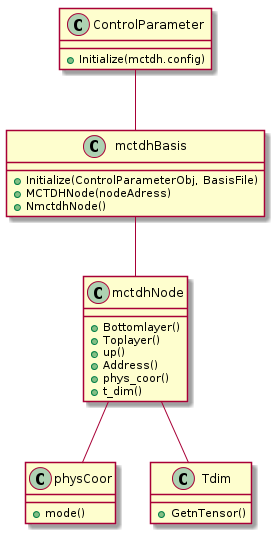
\includegraphics[scale=0.6]{figures/sequenceDiagram}
    \caption{Alle Klassen, die in Cython erstellt wurden, sind mit einem ,,C'' gekennzeichnet. Die jeweiligen Klassenmethoden sind mit einem
    gr"unen Punkt gekennzeichnet.}\label{fig:uml_Cython}
\end{figure}

\section{Graphische Benutzeroberfl"ache f"ur MCTDH}

 Die graphisch Benutzeroberfl"ache (GUI) f"ur MCTDH-Rechnungen wurde in Python und Qt implementiert.
 Der Zugriff auf die Qt-Bibliothek erfolgt "uber die Python-Bibliothek PyQt4. 
 PyQt4 umfasst zehn Python-Module, die zusammen ungef"ahr 400 Klassen und 6000 Methoden und Funktionen enthalten. \cite{PyQt}

 \begin{figure}
    \centering
    \vspace*{-0.5cm}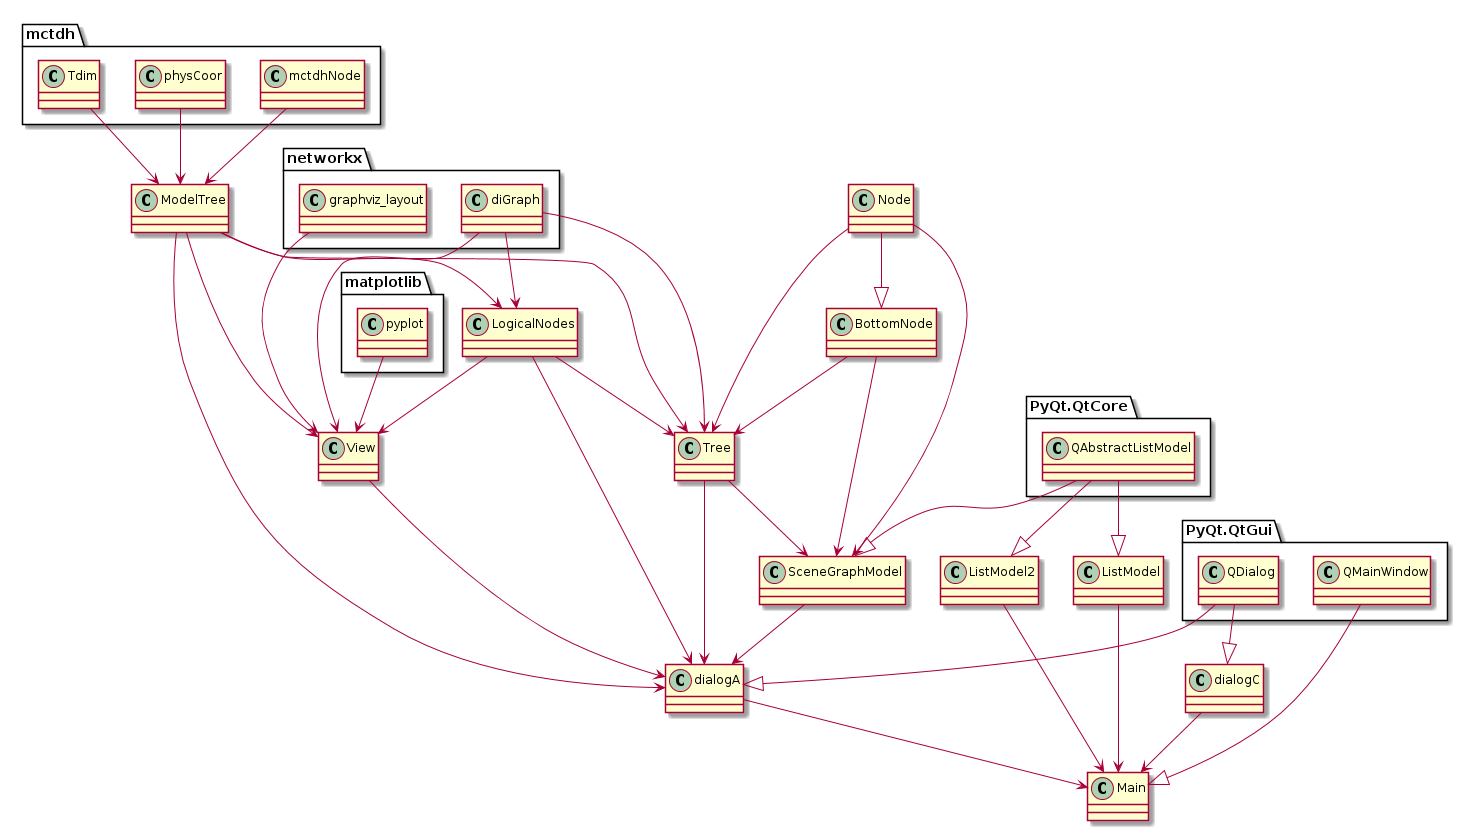
\includegraphics[width=\textwidth, angle=90, scale=1.4]{figures/umlPyQt}
    \caption{Klassendiagram der MCTDH-GUI. Eine Beschreibung des Diagramms
     findet sich im Text wieder.}\label{fig:uml_PyQt}
\end{figure}

In Abbildung \ref{fig:uml_PyQt} sind die wichtigen Klasse aufgef"uhrt, die f"ur die Implementierung der GUI verwendet wurden. 
Die Klassen, die in Rechtecken zusammengefasst wurden, entstammen aus Python-Modulen, deren Namen links "uber den Rechtecken angegeben sind.
Bei den Modulen handelt es sich um die PyQt4-Module \textit{QtCore} und \textit{QtGui}. F"ur die graphisch Darstellung der MCTDH-Baumdiagramme
wurden die Module \textit{matplotlib} und \textit{networkx} verwendet. Die Klassen, die in Abschnitt \ref{sec:PyInterface} vorgestellt wurden,
sind im Modul \textit{mctdh} enthalten. 

Alle \textit{mctdh}-Klassen werden in ModelTree verwendet, um alle Informationen zum MCTDH-Baum zu erhalten. Die Information wird an die
Klasse \textit{LogicalNodes} "ubergeben und es werden in dem Datentyp \textit{Dictionary} die Knoten des Baums mit den SPFs und f"ur den 
untersten Layers mit den Moden gespeichert. Speziell f"ur die Visualisierung von Baumdiagramme existiert das Python-Modul \textit{networkx}, 
aus dem die Klasse \textit{diGraph} verwendet wird, in der die Knoten gespeichert werden. Das Baumdiagramm wird in der Klasse \textit{View}
in einem \textit{png}-File mithilfe des Moduls \textit{matplotlib} gespeichert, das f"ur die Erzeugung von Diagrammen entwickelt wurde.
Das \textit{png}-File wird anschlie"send in der GUI verwendet. Die Informationen "uber den MCTDH-Baum wird von \textit{LogicalNodes}
auch an die Klasse \textit{Tree} "ubergeben.

Die Pfeile mit den ausgef"ullten Pfeilk"opfen  f"uhren von Klassen, die in anderen Klassen verwendet werden,
auf die die Pfeilspitze zeigt. 
Auf die Klassen, die durch Vererbung erstellt wurden, zeigen rot umrandete Pfeilspitzen. Beispielswei"se f"uhren diese Pfeile von allen angegeben PyQt-Klassen
, von denen geerbt wird.
Sowohl von \textit{QDialog} als auch \textit{QMainWindow} werden durch Vererbung Unterklassen generiert: \textit{dialogA, dialogc} und \textit{Main}. 
Allerdings wurden diese drei Klassen in Qt-Designer erzeugt, in dem die jeweiligen Fenster mit den ben"otigten Steuerungselementen zusammengestellt werden 
k"onnen. So k"onnen die Gr"o"sen der Steuerungselemente ohne Programmierung per Maus festgelegt werden. Die Informationen "uber 
die jeweiligen Fenster werden in \textit{ui}-Dateien gespeichert. Mit PyQt k"onnen diese Dateien eingelesen werden und aus den Daten die entsprechenden 
Klassen erstellt und beliebig erweitert werden.
Die beiden Klassen\textit{QDialog} und \textit{QMainWindow} stammen von \textit{QWidget} ab. \textit{QWidget}, \textit{QDialog} und \textit{QMainWindow}
sind Steuerungselement, mit denen der Benutzer durch die Tastatur und Maus interagieren kann. \cite{PyQt}

Die Klasse \textit{Main} stellt das Hauptfenster der GUI dar, von dem aus neue Projektordner erstellt, umbenannt oder gel"oscht werden k"onnen.
In diesen Ordner finden sich wiederum Ordner, die Einstellungen unterschiedlicher Rechnungen enthalten. Schlie"slich k"onnen aus
dem Hauptfenster neben der Ordernderverwaltung MCT\-DH-Rechnungen gestartet werden.
Die Klasse \textit{dialogC} generiert eine Fenster, in dem die Ordnernamen eingetragen werden k"onnen, um entweder neue Ordner zu erstellen
oder alte Ordner um zu benennen.
Die Einstellungsparameter einer MCTDH-Rechnung werden in der Klasse \textit{dialogA} angegeben. Bereits existierende MCTDH-Basisfiles werden
eingelesen und im \textit{dialogA}-Fenster dargestellt.


Alle Steuerungselement wie Kn"opfe, Checkboxen oder Elemente innerhalb eines Fensters emittieren Signale aus, die Aktionen des Benutzers
zugeordnet werden k"onnen. Aktionen k"onnen das Einmal- oder Doppeltklicken, das Bewegen des Mauszeigers oder das Bet"attigen der Entertaste sein.
Einzelne Steuerungselemente k"onnen zusammen mit einer bestimmten Aktion mit einer Klassenmethode bzw. Funktion verbunden werden, die die Klassenmethoden ausl"osen. 
  

Qt enth"alt Klassen, mit denen beliebig viele Elemente dargestellt werden k"onnen. Diesen Klassen liegt eine Model/View-Aufbau zugrunde,
 der das Datenmodel von der Darstellung der Daten trennt. 
Ein Datenmodel ist die Klasse \textit{QAbstractListModel}, in die die Daten eingelesen, bearbeitet und gel"oscht werden k"onnen.
Die Daten k"onnen wiederum in den Klassen \textit{QListView} und \textit{QTreeView} dargestellt werden. 
Die Trennung zwischen dem Datenmodel und der graphischen Darstellung der Daten beruht auf dem Model-View-Controller (MVC) Paradigma.\cite{Qt}  

Bei der MVC-Programmierung werden verschiedener Klassen erstellt. Jede dieser Klassen erf"ullt unterschiedliche Aufgaben:
die Verarbeitung von Daten innerhalb der
Anwendungssoftware (Model), die Visualisierung des aktuellen Systemzustandes (View) und die Interaktion zwischen Benutzer und Programm (Controller). \cite{MVC}

In Qt wurden der Controller und View kombiniert, sodass die Speicherung und Bearbeitung der Daten  von der Datenvisualisierung  
getrennt wurde. Die gleichen Daten k"onnen in verschieden Ansichten dargestellt werden. 
Die Implementierung neuer Darstellungsarten "andert nicht die darunterliegende Datenstruktur.\cite{Qt} 
Der Vorteil der Model/View-Architektur ist, dass die Element, die die visualisierten Daten des Models darstellen, nicht jeweils mit einer
Funktion gekoppelt werden muss wie bei anderen Steuerungselementen. So k"onnen Aktionen beliebig vieler Elemente 
mit nur einer Funktion verbunden werden. Dabei wird nur das Steuerungselement, das die Daten darstellt, mit den gew"unschten
Aktionen verbunden, wobei Aktionen auf ein beliebiges Element innerhalb der Steuerungselemente Informationen "uber dieses Element 
in Bezug auf das Datenmodel an die Funktion "ubertr"agt.

Qt besitzt f"ur die Model/View-Architektur Standardmodel, allerdings k"onnen die Modelle durch die Vererbung
von QAbstractListModel ver"andert und angepasst werden. So bekommt \textit{SceneGraphModel} keine Liste als Eingabetype wie die Klassen \textit{ListModel} und
\textit{ListModel2},
sondern Objekte der Klassen \textit{Node} und \textit{BottomNode}. 
Die Klasse \textit{BottomNode} erbt von \textit{Node} und enth"alt zus"atzlich Informationen zu den Moden der untersten Knoten. 
\textit{Node}-Objekte spiegeln bestimmte Knoten des
MCTDH-Baums wieder, in denen Informationen zu Elternknoten und Kinderknoten gespeichert sind. Diese Objekte werden
in der Klasse \textit{Tree} in einem \textit{Dictionary} zum Baum zusammengefasst. 
Die Daten des Models aus \textit{SceneGraphModel} werden "uber die PyQt-Klasse QTreeView in \textit{dialogA} visualisiert.
\textit{ListModel} und \textit{ListModel2} enth"alt eine Liste der Projektordner und der Ordner verschiedener Rechnungen innerhalb der Projekte.
Diese Daten werden in zwei getrennten QListView dargestellt und k"onnen mithilfe des Models aktualisiert werden.




  




   

     \chapter{Fazit und Ausblick}

in dieser Arbeit wurde ein MCTDH-Python-Modul erstellt, das Klassen des MCTDH-Codes in Python nutzbar macht.
In Zukunft k"onnten weitere Teile des MCTDH-Codes in Python zug"anglich gemacht werden, sodass weitere Features 
des MCTDH-Codes in Python verwendet werden kann.
Es w"are denkbar, dass n"utzliche Python-Module wie NumPy (numerical Python), SciPy (Scientific Computing Tools for Python)\cite{SciPy}
und TensorFlow (machine learning) \cite{TensorFlow} nahtlos mit dem MCTDH-Modul genutzt werden k"onnte. 

Auch die MCTDH-GUI kann erweitert werden. Eine Auswahl an Basisdateien f"ur verschiedene Hamiltonoperatoren existiert bereits. Der n"achste Schritt
w"are die M"oglichkeit, dass der Benutzer die Hamiltonoperatoren durch das Anklicken vorgegebener Terme selber erstellt. 
Des Weiteren k"onnte ein Ausgabefenster erstellt werden, das die Zwischenergebnisse w"ahrend der MCTDH-Rechnung graphisch darstellt.
Schlie"slich w"are auch das Implementieren der MCTDH-GUI als App auf Smartphones f"ur die Benutzer hilf\-reich, von dem sie die laufenden Rechnungen
"uberpr"ufen k"onnten. 
%	 \input{./content/dis}
%     \input{./content/Diskussion}

% ---------------------------------------------------------------
\backmatter % ab hier keine Nummerierung mehr
    \appendix
    \chapter{Anhang: Quellcode der GUI}

Der Quellcode der Python-Klassen, die f"ur die Erstellung der GUI genutzt wurden, wurde in verschiedenen 
Python-Dateien gespeichert. Im Folgenden werden die Dateinamen und der dazugeh"orige Quellcode aufgef"uhrt:

\vspace{5mm}

dialogC.py:
\begin{verbatim}
    from PyQt4 import QtCore, QtGui, uic
    import sys, os
    from widgetA import WidgetA
    
    base, form = uic.loadUiType("dialogNewName.ui")
    
    class DialogC(base, form):
        def __init__(self, parent=None):
            super(base, self).__init__(parent)
            self.setupUi(self)
    
            self._FolderName = ""
            self._cancel = None
    
            self.uiWarning.setText('')
            self.uiFolderName.setText("Give name for new Folder!")
            self.uiFolderName.selectAll()
            self.uiFolderName.textChanged.connect(self.change0)
            self.uiSaveBu.clicked.connect(self.save)
            self.uiCancelBu.clicked.connect(self.esc)
        
        def setWarning(self, warningUi):
            print warningUi
            self.uiWarning.setText(warningUi)
    
        def save(self):
            self._FolderName = self.uiFolderName.text()
            if ' ' not in self._FolderName:
                self.close()
            else:
                self.setWarning(str('Name contains whitespace'))
                print 'Name contains whitespace'
    
        def esc(self):
            self._cancel = "Cancel"
            self.close()
    
        def change0(self):
            self._FolderName = self.uiFolderName.text()
\end{verbatim}

InputPro.py:

\begin{verbatim}
from PyQt4 import QtCore, QtGui
import sys, os

class ListAbstrModel(QtCore.QAbstractListModel): 
    def __init__(self, data=[], parent=None):
        super(ListAbstrModel, self).__init__(parent)
        self.__data = data

    def rowCount(self, parent):
        return len(self.__data)

    def data(self, index, role):
        if role == QtCore.Qt.EditRole:
            row = index.row()
            return self.__data[row]

        if role == QtCore.Qt.DisplayRole:
            row = index.row()
            value = self.__data[row]
            return value

    def flags(self, index):
        return QtCore.Qt.ItemIsEditable |QtCore.Qt.ItemIsEnabled 
        |QtCore.Qt.ItemIsSelectable

    def setData(self, index, value, role=QtCore.Qt.EditRole):
        if role == QtCore.Qt.EditRole:
            row = index.row()
            self.__data[row] = str(value.toString())
            return True
        return False

class ListModel(ListAbstrModel):
    def __init__(self, data=[], parent=None):
        super(ListModel, self).__init__(data, parent)
        self.__data = data
        self.__dataBefore = list(data)
        self._messageBu = False

    def setData(self, index, value, role=QtCore.Qt.EditRole):
        if value not in self.__data:
            if role == QtCore.Qt.EditRole:
                row = index.row()
                self.__data[row] = str(value.toString())
                self.getValue()
                return True
        else:
            return False

    def getValue(self):
        matches = list(set(self.__data).intersection(self.__dataBefore))
        new = [l_ for l_ in self.__data if l_ not in matches]
        old = [l_ for l_ in self.__dataBefore if l_ not in matches]
        print new, old
        print os.getcwd()
        self.__dataBefore = list(self.__data)
        try:
            os.rename(old[0], new[0])
        except OSError:
            raise

    def removeRows(self, position, rows, parent=QtCore.QModelIndex()):
        self.beginRemoveRows(parent, position, position+rows-1)

        value = self.__data[position]
        self.showdialog(value)
        if self._messageBu == 'OK':
            for i in range(rows):    
                value = self.__data[position]   
                self.__data.remove(value)
            self.endRemoveRows()
            return True
        else:
            self.endRemoveRows()
            return False
            
    def showdialog(self, value):
        msg = QtGui.QMessageBox()
        msg.setIcon(QtGui.QMessageBox.Warning)

        msg.setText("Are sure you want to delete Folder %s?" %value)
        msg.setStandardButtons(QtGui.QMessageBox.Ok| QtGui.QMessageBox.Cancel)

        msg.buttonClicked.connect(self.msgbtn)
        msg.exec_()

    def msgbtn(self, i):
        self._messageBu = str(i.text())
        
class ListModel2(ListModel):  
    def __init__(self, project, data=[], parent=None):
        super(ListModel2, self).__init__(data, parent)
        self.__data = data
        self.__dataBefore = list(data)
        self._changePath = os.getcwd() + '/' + project

    def setData(self, index, value, role=QtCore.Qt.EditRole):
        if value not in self.__data:
            if role == QtCore.Qt.EditRole:
                row = index.row()
                self.__data[row] = str(value.toString())
                self.getValue(row)
                return True
        else:
            return False

    def getValue(self, row):
        matches = list(set(self.__data).intersection(self.__dataBefore))
        new = [l_ for l_ in self.__data if l_ not in matches]
        old = [l_ for l_ in self.__dataBefore if l_ not in matches]
        self.__dataBefore = list(self.__data)
        os.chdir(self._changePath)
        try:
            os.rename(old[0], new[0])
        except Exception:
            self.showdialog(row)

    def removeRows(self, position, rows, parent=QtCore.QModelIndex()):
        self.beginRemoveRows(parent, position, position+rows-1)

        value = self.__data[position]
        for i in range(rows):    
            value = self.__data[position]   
            self.__data.remove(value)
        self.endRemoveRows()
        return True
\end{verbatim}

InputTree.py:

\begin{verbatim}
##############################################################    
#    Title: PyQt4 Model View Tutorial Part 04
#    Author: Yasin Uludag
#    Date: 2011
#    Availability: https://www.youtube.com/watch?v=pr1M3mP7qfI
##############################################################

from PyQt4 import QtCore, QtGui, uic
import sys
from Node import Node, BottomNode, Tree

class SceneGraphModel(QtCore.QAbstractItemModel):
    def __init__(self, root, parent=None):
        super(SceneGraphModel, self).__init__(parent)
        self._rootNode = root
        self._child = None
        self._childIndex = QtCore.QModelIndex()
        self._dictNodes = {}

    def parent(self, index):
        node = index.internalPointer()
        parentNode = node.parent()

        if parentNode == self._rootNode:
            return QtCore.QModelIndex()
        return self.createIndex(parentNode.row(), 0, parentNode)

    def index(self, row, column, parent):


        childItem = parentNode.child(row)

        if childItem:
            return self.createIndex(row, column, childItem)
        else:
            return QtCore.QModelIndex()

    def rowCount(self, parent):
        if not parent.isValid():
            parentNode = self._rootNode
        else:
            parentNode = parent.internalPointer()

        return parentNode.childcount()

    def columnCount(self, parent):
        return 2

    
    def flags(self, index):
        return QtCore.Qt.ItemIsEnabled | QtCore.Qt.ItemIsSelectable | \
            QtCore.Qt.ItemIsEditable | QtCore.Qt.ItemIsDragEnabled | \
            QtCore.Qt.ItemIsDropEnabled

    def headerData(self, section, orientation, role):
        if role == QtCore.Qt.DisplayRole:
            if section == 0:
                return "Node"
            else:
                return "Mode"

    def data(self, index, role):

        if not index.isValid():
            return None

        node = index.internalPointer()

        if role == QtCore.Qt.DisplayRole or role == QtCore.Qt.EditRole:
            if index.column() == 0:
                return node.name()
            else:
                if node.typeInfo() == "Bottom":
                    return node._physcoor

        if role == QtCore.Qt.DecorationRole:
            if index.column() == 0:

                typeInfo = node.typeInfo()

    def setData(self, index, value, role = QtCore.Qt.EditRole):
        if index.isValid():
            if role == QtCore.Qt.EditRole:
                node = index.internalPointer()
                if index.column() == 0:
                    node.setName(str(value.toString()))
                    return True
                elif index.column() == 1:
                    node.setPhyscoor(str(value.toString()))
                    return True
        return False

    def getNode(self, index):
        if index.isValid():
            node = index.internalPointer()
            if node:
                return node
        return self._rootNode

    def getNode2(self, index):
        return self._rootNode

    def insertRows(self, position, rows, parent=QtCore.QModelIndex()):
        parentNode = self.getNode(parent)
        oldNode = self._child
        if oldNode.typeInfo() == 'NODE':
            self.addNode(oldNode.name(), oldNode.name(), None)    
        if oldNode.typeInfo() == 'Bottom':
            self.addBottomNode(oldNode.name(), oldNode.name(), None, \
            oldNode.physcoor())
        self.copyNode(self._child)

        self.beginInsertRows(parent, position, position+rows-1)

        for row in range(rows):
            success = parentNode.insertChild(position, \
            self._dictNodes[oldNode.name()])  

        self.endInsertRows()

        return success

    def removeRows(self, position, rows, parent=QtCore.QModelIndex()):
        parentNode = self.getNode(parent)
                
        self.beginRemoveRows(parent, position, position+rows-1)

        for row in range(rows):
            
            success = parentNode.removeChild(position)

        self.endRemoveRows()

        return success

#####Drag and Drop######

    def supportedDropActions(self):
        return QtCore.Qt.CopyAction | QtCore.Qt.MoveAction

    def mimeTypes(self):
        types = QtCore.QStringList()
        types.append('text/plain')
        return types

    def mimeData(self, index):  
        rc = ''
        self._child = index[0].internalPointer()
        self._childIndex = index[0]
        mimeData = QtCore.QMimeData()
        mimeData.setText(rc)
        return mimeData

    def dropMimeData(self, data, action, row, column, parentIndex):
        if action == QtCore.Qt.IgnoreAction:
            return True
        
        self.insertRows(0,1, parentIndex)
        index = self._childIndex
        self.removeRows(0,1, index)
        print self._rootNode.child(0)
        return True

    def copyNode(self, oldNode):
        children = oldNode.childAll()
        if children:
            for oldchild in children:
                if oldchild.typeInfo() == "NODE":
                    self.addNode(oldchild.name(), oldchild.name(), \
                    self._dictNodes[oldNode.name()])
                if oldchild.typeInfo() == "Bottom":
                    self.addBottomNode(oldchild.name(), oldchild.name(), \
                    self._dictNodes[oldNode.name()], oldchild.physcoor())
                self.copyNode(oldchild)
    
    def addNode(self, obj, SPF, parent):
        self._dictNodes[obj] = Node(SPF, parent)

    def addBottomNode(self, obj, SPF, parent, physcoor):
        self._dictNodes[obj] = BottomNode(SPF, parent, physcoor)
\end{verbatim}

LogicalNodes.py:

\begin{verbatim}
from ModelTree import ModelTree
import networkx as nx
from networkx.drawing.nx_agraph import write_dot, graphviz_layout
import matplotlib.pyplot as plt

class LogicalNodes():
    def __init__(self, layer_matr, config_file, sys_file):
        self.G = nx.DiGraph()
        self.layer_matr = layer_matr
        self.ModelTree = ModelTree(config_file, sys_file)
        self.label_mode = self.ModelTree.label_mode
        self.nodes_spf = self.ModelTree.nodes_spf
        self.Networkx()
        self.augDiGraph("SPF", self.nodes_spf)
        self.augDiGraph("Mode", self.label_mode)

    def Networkx(self):
        for c_ in self.layer_matr:
            for b_ in c_:
                self.G.add_node(b_)
                l = len(c_)
                for index, b_ in enumerate(c_):
                    if index < (l-1):
                        self.G.add_edge(b_, c_[index + 1], weight=1)

    def augDiGraph(self, str_kind, str_dict):
        for key, ele_ in str_dict.items():
            self.G.nodes[key][str_kind] = ele
\end{verbatim}

main.py:

\begin{verbatim}
    from PyQt4 import QtGui, QtCore, uic
    import sys, os, shutil
    from widgetA import WidgetA
    from InputPro import ListModel, ListModel2
    from dialogC import DialogC
    from dialogD import DialogD
    
    
    base, form = uic.loadUiType("main.ui")
    
    class Main(base, form):
        def __init__(self, parent=None):
            super(base, self).__init__(parent)
            self.setupUi(self)
    
            self._HamiltonianDir = os.getcwd() + '/' + 'Hamiltonians'
            os.chdir('Projects')
            self._startingPath = os.getcwd()
            self._ProjectName = None
            self._path2 = None
            self._dir_list = None
            self._proContent = []
    
            self._model1 = None
            self._model2 = None
            self._itemIndex1 = None
            self._itemIndex2 = None
    
            self.getdirs()
            self._WidgetA = WidgetA(self)
            self._WidgetA._HamiltonianDir = self._HamiltonianDir
            self._WidgetA._startingPath = self._startingPath
    
            self.setList()
            self.uiNew.triggered.connect(self.openA)
            self.uiLoad.triggered.connect(self.openB)
            self.uiMCTDHcalc.triggered.connect(self.openD)
            self.uiMCTDHexisting.triggered.connect(self.runJob)
            self.uiPlusBu.clicked.connect(self.openA)
            self.uiPlusBu2.clicked.connect(self.open0)
            self.uiMinusBu.clicked.connect(self.removeA)
            self.uiMinusBu2.clicked.connect(self.remove0)
    
            self.uiProjects.clicked.connect(self.on_item_select)
            self.uiProjects.customContextMenuRequested.connect(self.openMenu)
    
            self.setList2()
            self.uiSessions.clicked.connect(self.on_item_select0)
            self.uiSessions.customContextMenuRequested.connect(self.openMenu0)
    
            self._dialogD = DialogD()
    
            self._messageBu = None
    
        def openMenu0(self, position):
            """Context menu"""
            menu = QtGui.QMenu()
            renameAction = menu.addAction("Rename")
            action = menu.exec_(self.uiSessions.mapToGlobal(position))
            if action == renameAction:
                self.uiSessions.edit(self._itemIndex2)
    
        def openMenu(self, position):
            """Context menu"""
            menu = QtGui.QMenu()
            renameAction = menu.addAction("Rename")
            action = menu.exec_(self.uiProjects.mapToGlobal(position))
            if action == renameAction:
                self.uiProjects.edit(self._itemIndex1)
    
        def remove0(self):
            """Removes Rows from ListModel2()"""
            rowNum = self._itemIndex2.row()
            session = str(self._itemIndex2.data().toString())
            self.showdialog(session)
            if 'OK' in self._messageBu:
                self._model2.removeRows(rowNum,1, self._itemIndex2)
    
                shutil.rmtree(self._startingPath+'/'+self._ProjectName+'/'+session)
    
        def removeA(self):
            """Removes Rows from ListModel()"""
            rowNum = self._itemIndex1.row()
            key = str(self._itemIndex1.data().toString())
            startingpath2 = self._startingPath + '/'
            delFolder = startingpath2 + key
    
            self._model1.removeRows(rowNum,1, self._itemIndex1)
    
            if self._model1._messageBu == 'OK' and delFolder != self._startingPath 
            and delFolder != startingpath2:
                shutil.rmtree(self._startingPath+'/'+key)
    
                maxRow = self._model2.rowCount(self._itemIndex2)
                if maxRow != 0:
                    self._model2.removeRows(0, maxRow)
    
        def showdialog(self, value):
            msg = QtGui.QMessageBox()
            msg.setIcon(QtGui.QMessageBox.Warning)
    
            msg.setText("Are sure you want to delete Folder %s?" %value)
            msg.setStandardButtons(QtGui.QMessageBox.Ok| QtGui.QMessageBox.Cancel)
    
            msg.buttonClicked.connect(self.msgbtn)
            msg.exec_()
    
        def msgbtn(self, i):
            self._messageBu = str(i.text())
    
        def getContent(self):
            os.chdir(self._startingPath)
            if os.path.exists(self._ProjectName):
                directories = os.walk('./'+self._ProjectName).next()[1]
                try:
                    directories.remove('tmp') 
                except ValueError:
                    pass
                self._proContent = sorted(directories)
            else:
                print("path doesn't exists")
    
        def on_item_select0(self, index):
            """clicked Event on Items belonging to ListModel2()"""
            os.chdir(self._startingPath)
            projectFolder = str(self._itemIndex1.data().toString())
            sessionFolder = str(index.data().toString())
            self._itemIndex2 = index
            self._ProjectName = projectFolder
    
            os.chdir(self._ProjectName)
            self._WidgetA._ProjectName = projectFolder
            self._WidgetA.makedir()
            self._WidgetA.editSession(sessionFolder)
            self._WidgetA.setSessionName(sessionFolder)
            self._WidgetA.start()
            self._WidgetA.removeContent()
            SESfiles = os.walk(self._startingPath+'/'+self._ProjectName+'/'
            +sessionFolder).next()[2]
            if SESfiles:
                for f_ in SESfiles:
                    if 'txt' in f_:
                        self._WidgetA.fromSESToTMP(f_)
            self.openC()
            os.chdir('./')
    
        def on_item_select(self, index):
            """clicked Event on Items belonging to ListModel()"""
            self._itemIndex1 = index
            self._ProjectName = str(index.data().toString())
            self._WidgetA._ProjectName = self._ProjectName
            self._WidgetA._SessionName = None
            self._WidgetA.clearSession()
            self.getdirs()
            self.setList2()
    
        def setList2(self):
        #####ListModelPES#######
            self.getContent()
            self._model2 = ListModel2(self._ProjectName, self._proContent)
            self.uiSessions.setModel(self._model2)
            indices = self.uiSessions.selectionModel().selectedIndexes()
            if not indices:
                index = self._model2.index(0,0)
                self._itemIndex2 = index
                self.uiSessions.selectionModel().select(index, /
                QtGui.QItemSelectionModel.Select)
                self._path2 = str(self._itemIndex2.data().toString())
    
        def setList(self):
        #####ListModelPES#######
            self.getdirs() 
            self._model1 = ListModel(self._dir_list)
            self.uiProjects.setModel(self._model1)
            indices = self.uiProjects.selectionModel().selectedIndexes()
            if not indices:
                index = self._model1.index(0,0)
                self._ProjectName = str(index.data().toString())
                self._WidgetA._ProjectName = self._ProjectName
                self._itemIndex1 = index
                self._itemProxyIndex1 = index
                self.uiProjects.selectionModel().select(index, /
                QtGui.QItemSelectionModel.Select)
    
        def getdirs(self):
                directories = os.walk(self._startingPath).next()[1]
                self._dir_list = [dirs for dirs in directories]
                self._dir_list = sorted(self._dir_list)
    
        def open0(self, warn):
            if warn == False:
                warn = ''
            dialogC = DialogC()
            dialogC.setWarning(str(warn))
            dialogC.exec_()
            self._path2 = str(dialogC._FolderName)
            print self._path2
    
            if str(dialogC._cancel) != 'Cancel':
                path = self._startingPath + '/' + self._ProjectName + '/' 
                + self._path2
                if not os.path.exists(path):
                    try:
                        os.chdir(self._startingPath+'/'+self._ProjectName)
                        os.makedirs(self._path2)
                        os.chdir(self._startingPath)
                    except IOError as identifier:
                        print (dir(identifier))
                    self.getContent()
                    self.setList2()
                else:
                    print('Folder already exists!')
                    self.open0('Folder already exists!')
    
        def openA(self, warnings):
            if warnings == False:
                warnings = ''
            dialogC = DialogC()
            dialogC.setWarning(str(warnings))
            dialogC.exec_()
            self._ProjectName = str(dialogC._FolderName)
    
            if self._ProjectName != 'Cancel':
                path = self._startingPath + '/' + self._ProjectName
   
                if not os.path.exists(path):
                    try:
                        os.makedirs(path)
                        os.makedirs(path+'/tmp')
                    except IOError as identifier:
                        print (identifier)
   
                    self.setList()
                else:
                    print('Folder already exists!')
                    self.openA('Folder already exists!')
    
        def openB(self):
            self._ProjectName = str(QtGui.QFileDialog.getExistingDirectory(self))
            self._ProjectName = self._ProjectName.split("/")[-1]
            self.getContent()
            self.setList2()
    
        def openC(self):
            dialog = self._WidgetA
            dialog.exec_()
            self.setList2()
    
        def openD(self):
            self._WidgetA.clearSession()
            self._WidgetA.setSessionName(None)
            self._WidgetA.removeContent()
    
            self.openC()
    
        def Finder(self, path, app):
            fileList = os.walk(path).next()[2]
            return [f_ for f_ in fileList if app in f_][0]
    
        def getRunInput(self):
            filePathList = []
            self.getContent()
            self._proContent
            for root, dirs, files in os.walk(self._startingPath+'/'
            +self._ProjectName):
                for name in files:
                    filePathList.append(os.path.join(root, name))
            filePathList = [p_ for p_ in filePathList if '.in' in p_]
            filePathList = [f_.split('/')[-2:] for f_ in filePathList]
            filePathList = [f_ for f_ in filePathList if f_[0] in self._proContent]
            return ['/'.join(f_) for f_ in filePathList]
    
        
    
        def runJob(self):
            '''Try QProcess from Qt'''
            dialog = self._dialogD
            self._dialogD._model = QtGui.QStandardItemModel(self._dialogD.uiRunList)
            self._dialogD.uiRunList.setModel(self._dialogD._model)
            self._dialogD.uiRunList.setEditTriggers(QtGui.QAbstractItemView.
            NoEditTriggers)
            inputList = self.getRunInput()
    
            for calc in inputList:
                item = QtGui.QStandardItem(calc)
                self._dialogD._model.appendRow(item)
    
            self._dialogD.uiRunList.clicked.connect(self.on_item_select2)
            dialog.exec_()
            
    
        def on_item_select2(self, index):
            inputFile = self._startingPath+'/'+self._ProjectName+'/'
            +str(index.data().toString())
    
            self.process = QtCore.QProcess()
            self.process.setProcessChannelMode(QtCore.QProcess.MergedChannels)
            self.process.readyReadStandardOutput.connect(self.mctdhOut)
            self.results(inputFile)
    
        def results(self, inputFile):
            os.chdir('../Results')
            self._WidgetA.genereInput(inputFile)
            try:
                os.mkdir(self._WidgetA._mainfolder)
            except OSError:
                pass
            mctdh = '/home/piet/newRepo/QuantumDynamics/build/bin/mctdh'
            self.process.start(mctdh+' '+inputFile)
            os.chdir(self._startingPath)
            self._dialogD.close()
    
        def mctdhOut(self):
            output = str(self.process.readAllStandardOutput())
            print output
    
    if __name__ == '__main__':
    
        app = QtGui.QApplication(sys.argv)
        app.setStyle("cleanlooks")
        wnd =Main()
        wnd.show()
        sys.exit(app.exec_())
\end{verbatim}

ModelTree.py:

\begin{verbatim}
    import mctdh
    import sys
    
    class ModelTree(object):
        def __init__(self, config_file='mctdh.config', sys_file='CH3g1.txt'):
            self.config_file = config_file
            self.sys_file = sys_file
            self.bottom_list = []
            self.mode_list =[]
            self.layer_list = []
            self.layer_matr = []
            self.lay_matr_mode = []
            self.label_mode = {}
            self.nodes_spf = {}
    
            print self.config_file, 'from ModelTree'
            print self.sys_file, 'from ModelTree'
            self.config = mctdh.controlParameters()
            self.config.initialize(self.config_file)
            self.basis = mctdh.MctdhBasis()
            self.basis.initialize(self.sys_file, self.config)
            self.node = mctdh.MctdhNode()
            self.phys = mctdh.PhysCoor()
            self.tdim = mctdh.Tdim()
    
            self.getLayerMatr()
            self.getPhysCoord()
            self.modeToGetLayer()
            self.get_SPFs()
    
    
        def getBottomlayer(self):
            """Get the bottom nodes"""
            for i in range(self.basis.NmctdhNodes()):
                self.node = self.basis.MCTDHnode(i)
                if self.node.Bottomlayer() == True:
                    self.bottom_list.append(i)
            return self.bottom_list #List of the i-th bottom node
    
        def getPhysCoord(self):
            """get the Modes of the pys. Coordinates"""
            for i in range(self.basis.NmctdhNodes()):
                self.node = self.basis.MCTDHnode(i)
                if self.node.Bottomlayer() == True:
                    self.phys = self.node.phys_coor()
                    self.mode_list.append(self.phys.mode()) #append Modes to list
    
        def nlayer(self, i):
            self.node = self.basis.MCTDHnode(i) #i-th Node
            self.layer_list.append(i)
            if self.node.Toplayer() == False:
                return self.nlayer(self.node.up().address())
            new_list = list(self.layer_list) #copy instead of reference
            del self.layer_list[:]
            return new_list
    
        def getLayerMatr(self):
            self.layer_matr = 
            [list(reversed(self.nlayer(b_))) for b_ in self.getBottomlayer()]
    
        def modeToGetLayer(self):
            self.lay_matr_mode = 
            [l_ + [100 + i] for i,l_ in enumerate(self.layer_matr)]
            self.lay_matr_mode = [["Top"] + l_ for l_ in self.lay_matr_mode]
            #concatinates two lists
            self.label_mode = [100 + i for i in range(len(self.mode_list))]
            self.label_mode = dict(zip(self.label_mode, self.mode_list))
    
        def get_SPFs(self):
            """get the SPFs of each Node"""
            for i in range(self.basis.NmctdhNodes()):
                self.node = self.basis.MCTDHnode(i)
                self.tdim = self.node.t_dim()
                self.nodes_spf[i] = self.tdim.GetnTensor() #dict
    
            mode_spf = [self.basis.MCTDHnode(i).t_dim().active(0) for i in \
                        range(self.basis.NmctdhNodes()) if \
                        self.basis.MCTDHnode(i).Bottomlayer() == True ]
    
            mode_spf_dict = dict(zip(self.label_mode, mode_spf))
            for k, i in zip(self.label_mode.keys(), mode_spf):
                self.nodes_spf[k] = i
\end{verbatim}

Node.py:

\begin{verbatim}
    from LogicalNodes import LogicalNodes
    from ModelTree import ModelTree
    import numpy as np
    import networkx as nx
    import re, sys, os
    
    class Parameters(object):
        def __init__(self):
            self._eps_general =  None
            self._eps_1 = None
            self._eps_2 = None
            self._start = None
            self._end = None
            self._dt = None
            self._iteration = None
            self._hamiltonian = None
            self._potential = None
            self._job = None
            self._parameters = None
            self._treeData = None
    
    class InPut(Parameters):
        def __init__(self, filename='example.in'):
            super(InPut, self).__init__()
            self._filename = filename
            self._filenameOld = None
            self._paradict = {}
            self._paralist = []
            self._treelist = []
            self._treeString = ''
            self._commDict = {}
            self.rmCommen()
            self.readFile()
    
        def readFile(self):
            self.getPara("mainfolder")
            self.getPara("Hamiltonian")
            self.getPara("Potential")
            self.getPara("job")
            self.getPara("start")
            self.getPara("end")
            self.getPara("dt")
            self.getPara("iteration")
            self.getPara("out")
            self.getPara2()
            self._paradict['para'] = self._paralist
            self._paradict['Comm'] = self._commDict
            self.getTree()
    
        def file_len(self, fname):
            with open(fname) as f:
                for i, l in enumerate(f):
                    pass
            return i+1
    
        def getPara2(self):
            lineNum = self.file_len(self._filename)
            with open(self._filename, "rb") as text:
                for line in text:
                    if "parameters" in line:
                        for i in range(lineNum):
                            try:
                                para = text.next()
                                if bool(re.search(r'\d', para)):
                                    para = para.split()     
                                    self._paralist.append(para)
                            except StopIteration:
                                pass
            lastLine = [x for x in self._paralist[-1] if x != ']']
            del self._paralist[-1]
            self._paralist.append(lastLine)
    
        def rmCommen(self):
            with open(self._filename, "r") as in_put:
                with open('new_InPut.in', 'wb') as output:
                    i = 0
                    for line in in_put:
                        i += 1
                        if '//' in line:
                            self._commDict[i-1] = line
                        else:
                            output.write(line)
    
            self._filename = 'new_InPut.in'              
    
    
        def getPara(self, para):
            with open(self._filename, "rb") as text:
                for line in text:
                    if para in line:
                        try:
                            pos = line.index('=')     
                            self._paradict[para] = line[pos+1:].strip()  
                        except ValueError:
                            pass
    
        def getTree(self):                
            lineNum = self.file_len(self._filename)
            with open(self._filename, "rb") as text:
                for line in text:
                    if 'tree' in line:
                        for i in range(lineNum):
                            try:
                                tree = text.next()
                                if ']' in tree:
                                    break
                                self._treelist.append(tree)
                            except StopIteration:
                                pass
            self._treeString = ''.join(self._treelist)
    
    class OutPut(Parameters):
        def __init__(self, tree, paradict, sysFile, filename="InPut.in"):
            self._mainfolder = paradict['mainfolder']
            self._start = paradict['start']
            self._end =paradict['end']
            self._dt = paradict['dt']
            self._out = paradict['out']
            self._iteration = paradict['iteration']
            self._hamiltonian = paradict['Hamiltonian']
            try:
                self._potential = paradict['Potential']
            except KeyError:
                self._potential = 'no Potential'
            self._job = paradict['job']
            self._parameters = paradict['para']
            self._formated = self.formatparameter()
            self._treeData = tree._treeData
            self._filename = filename
            self._sysFile = sysFile
    
        def savefile(self):
            with open(self._filename, "w") as text_file:
                text_file.write("{0}".format(self.bringAllTogether()))
    
        def savefile2(self):
            with open(self._sysFile, "w") as text_file:
                text_file.write("{0}".format(self.bringTreePara()))
    
        def formatparameter(self):
            output = ""
            A = self._parameters        
            output = '\n'.join(['    '.
            join(['{:4}'.format(item) for item in row]) for row in A])
            return output
    
        def bringAllTogether(self):
    
            output = "mainfolder = " + self._mainfolder + "\n" \
            "Hamiltonian = " + self._hamiltonian + "\n" \
            "Potential = " + self._potential + "\n" \
            "\n" \
            "job = " + self._job + "\n" \
            "\n" \
            "integrator = { \n" \
            "start = " + self._start + "\n" \
            "end = " + self._end + "\n" \
            "dt = " + self._dt + "\n" \
            "iteration = " + self._iteration + "\n" \
            "out = " + self._out + "\n" \
            "} \n" \
            "\n" \
            "basis = \n" \
            "{\n" \
            "tree = [ \n" \
             + self._treeData + \
            "]\n" \
            "\n" \
            "\n" \
            "parameters = [\n" \
            + self._formated + \
            "]\n" \
            "}"
            return output
    
        def bringTreePara(self):
            output =  self._treeData + \
            "\n" \
            + self._formated
            return output
    
        def __repr__(self):
            return self.bringAllTogether()
    
    class OutPut2(object):
        def __init__(self, paradict, treeString, filename, pathTMP):
            self._parameters = paradict['para']
            self._formated = self.formatparameter()
            self._treeString = treeString
            self._sysFile = pathTMP + '/Load.txt'
            self._TMPmctdhConfig = pathTMP + '/mctdh.config'
            self._path = pathTMP
    
        def savefile(self):
            with open(self._TMPmctdhConfig, "w") as text_file:
                text_file.write("{0}".format(self.bringAllEPS()))
    
        def savefile2(self):
            with open(self._sysFile, "w") as text_file:
                text_file.write("{0}".format(self.bringTreePara()))
    
        def bringAllEPS(self):
            epsList = ['1E-6', '8E-5', '5E-5', '5E-5', '0', '0']
            output = '\n'.join(epsList)
            return output
    
        def bringTreePara(self):
            output =  self._treeString + \
            "\n" \
            + self._formated
            return output
    
        def formatparameter(self):
            output = ""
            A = self._parameters        
            output = '\n'.join(['    '.
            join(['{:4}'.format(item) for item in row]) for row in A])
    
            return output
    
    
    class Tree(object):
        def __init__(self, mctdhConfig, sys_file):
            self._rootNode0 = Node("TOP")
            self._dictNodes = {}
    
            model = ModelTree(mctdhConfig, sys_file)
            logical = LogicalNodes(model.lay_matr_mode, mctdhConfig, sys_file)
            self._G = logical.G
            self._elder = None
            self.getElder()
            self.addNode(self._elder, str(self._G.nodes[self._elder]['SPF']), 
            self._rootNode0)
            self.readTree()
    
            self._rootNode = self._dictNodes[self._elder]
            self._treeData = self._dictNodes[self._elder].log()
    
        def getElder(self):
            for ele_ in self._G.nodes():
                if self._G.pred[ele_] == {}:
                    self._elder = ele_
            self._elder = self._G.successors(self._elder).next()
    
    
        def readTree(self):
            for suc_ in nx.bfs_successors(self._G, self._elder):
                for brothers in suc_[1]:
                    if 'Mode' in self._G.nodes[brothers].keys():
                        self.addBottomNode(brothers, 
                        str(self._G.nodes[brothers]['SPF']), 
                        self._dictNodes[suc_[0]], 
                        str(self._G.nodes[brothers]['Mode']))
                    else:
                        self.addNode(brothers, str(self._G.nodes[brothers]['SPF']), 
                        self._dictNodes[suc_[0]]) #Label, SPF, parent_obj
    
        def setRootNode(self, rootNode):
            self._rootNode = rootNode
            self.setLog()
    
        def setLog(self):
            self._treeData = self._rootNode.log()
    
        def addNode(self, obj, SPF, parent):
            self._dictNodes[obj] = Node(SPF, parent)
    
        def addBottomNode(self, obj, SPF, parent, physcoor):
            self._dictNodes[obj] = BottomNode(SPF, parent, physcoor)





##############################################################    
#    Title: PyQt4 Model View Tutorial Part 04
#    Author: Yasin Uludag
#    Date: 2011
#    Availability: https://www.youtube.com/watch?v=pr1M3mP7qfI
##############################################################

    class Node(object):
        def __init__(self, name, parent=None):
            self._name = name
            self._children = []
            self._parent = parent
    
            if parent is not None:
                parent.addChild(self)
    
        def addChild(self, child):
            self._children.append(child)
    
        def insertChild(self, position, child):
            if position < 0 or position > len(self._children):
                return False
    
            self._children.insert(position, child)
            child._parent = self
            return True
    
        def removeChild(self, position):
            if position < 0 or position > len(self._children):
                return False
    
            try:
                child = self._children.pop(position)
                child._parent = None
                return True
            except IndexError as e:
                print e.message, ': from Node, 237'
                return False
    
        def name(self):
            return self._name
    
        def setName(self, name):
            self._name = name
    
        def child(self, row):
            return self._children[row]
    
        def childAll(self):
            return self._children
    
        def childcount(self):
            return len(self._children)
    
        def parent(self):
            return self._parent
    
        def row(self):
            if self._parent is not None:
                return self._parent._children.index(self)
    
        def log(self, tabLevel=-1):
            output = ""
            tabLevel += 1
    
            for i in range(tabLevel):
                output += "   "
            if self.childcount() == 0:
                output += self._name + "  " + str(self.childcount()) + "\n"
            else:
                output += self._name + " -" + str(self.childcount()) + "\n"
    
            for child in self._children:
                output += child.log(tabLevel)
    
            tabLevel -= 1
    
            return output
    
        def __repr__(self):
            return self.log()
    
        def typeInfo(self):
            return "NODE"
    
    class BottomNode(Node):
        def __init__(self, name, parent, physcoor):
            super(BottomNode, self).__init__(name, parent)
            self._physcoor = physcoor
    
        def typeInfo(self):
            return "Bottom"
    
        def physcoor(self):
            return self._physcoor
    
        def setPhyscoor(self, physcoor):
            self._physcoor = physcoor
    
        def log(self, tabLevel=-1):
            output = ""
            tabLevel += 1
    
            for i in range(tabLevel):
                output += "   "
            if self.childcount() == 0:
                output += self._name + "  " + str(self.childcount()) + 
                "   " + self._physcoor + "\n"
            else:
                output += self._name + " -" + str(self.childcount()) + "\n"
    
            for child in self._children:
                output += child.log(tabLevel)
    
            tabLevel -= 1
    
            return output
\end{verbatim}

View.py:

\begin{verbatim}
    import networkx as nx
    from networkx.drawing.nx_agraph import write_dot, graphviz_layout
    import matplotlib.pyplot as plt
    
    import sys
    from PyQt4 import QtGui
    
    
    class View(object):
        def __init__(self, label_mode, nodes_spf):
            self.label_mode = label_mode
            self.nodes_spf = nodes_spf
            self._G = nx.DiGraph()
        def Display(self, G):
            top = ['Top']
            rest_nodes = [l_ for l_ in self.nodes_spf.keys() 
            if l_ not in self.label_mode.keys()]
            pos = graphviz_layout(G, prog='dot')
            nx.draw(G, pos, with_labels=False, arrows=False, node_color='w')
            nx.draw_networkx_nodes(G, pos, nodelist=top, node_color='w', alpha=1)
            nx.draw_networkx_nodes(G, pos, nodelist=rest_nodes, node_color='r', 
            alpha=1)
    
            pos_lower = {}
            x_off = 0
            y_off = -5
            for k, v in pos.items():
                pos_lower[k] = (v[0] + x_off, v[1] + y_off)
    
            nx.draw_networkx_labels(G, pos_lower, self.label_mode, font_size=16)
    
            pos_higher = {}
            x_off = -7
            y_off = 27
            for k, v in pos.items():
                pos_higher[k] = (v[0] + x_off, v[1] + y_off)
    
            nx.draw_networkx_labels(G, pos_higher, self.nodes_spf, font_size=12)
            plt.savefig('nx_test.png')
            plt.clf()
    
            for key, ele_ in self.nodes_spf.items():
                G.nodes[key]["SPF"] = ele_
            for key, ele_ in self.label_mode.items():
                G.nodes[key]["Mode"] = ele_
            self._G = G
\end{verbatim}


widgetA.py:

\begin{verbatim}
    from PyQt4 import QtCore, QtGui, uic
    import sys
    from Node import OutPut, OutPut2, Tree
    from Node import InPut
    from InputTree import SceneGraphModel
    from ModelTree import ModelTree
    from LogicalNodes import LogicalNodes
    from View import View
    import os, shutil
    
    base, form = uic.loadUiType("dialogA.ui")
    
    class WidgetA(base, form):
        def __init__(self, parent=None):
            super(WidgetA, self).__init__(parent)
            self.setupUi(self)
    
            self._HamiltonianDir = None
            
            ########Attributes######
            self._paradict = {}
            self._integrator = []
            self._tree = None
            self._treeFromLoad = None
    
    
            self._dictHamil = {'CH3Quasie_exact': '1', 'CH4_rst': '2', 'NOCl': '9'}
            self._dictPES = {'CH3Potential': '1', 'PES_CH4': '2', 
            'PES_HCH4_Zang': '4'}
            self._potential = 'no Potential'
    
            self._mctdhConfig = None 
            self._sysTreeFile = None
            self._inputFile = None
            self._SESmctdhConfig = None
            self._SESsysTreeFile = None
            self._SESinputFile = None
            self._TMPmctdhConfig = None
            self._TMPsysTreeFile = None
            self._TMPinputFile = None
            self._dest = None
    
            self._startingPath = None
            self._ProjectName = None
            self._SessionName = None
            self._temporarySES = None
            self._messagebut = None
    
            #####ListModelHamilton#######
            self._model = QtGui.QStandardItemModel(self.listHamilton)
            for key in self._dictHamil:
                item = QtGui.QStandardItem(key)
                self._model.appendRow(item)
            self.listHamilton.setModel(self._model)
            self.listHamilton.setEditTriggers(QtGui.QAbstractItemView.
            NoEditTriggers)
            self.listHamilton.clicked.connect(self.on_item_select1)
    
            #####RadioButtonsPES#####
            self.onRadio.setChecked(True)
            self.onRadio.toggled.connect(self.setPES)
            self.offRadio.toggled.connect(self.unsetPES)
            self.offRadio.toggled.connect(self.noPotenial)
    
            #####ListView of PES is built###
            self.setPES()
    
            ###RadioButtonsJob####
            self.RealRadio.toggled.connect(self.setJob1)
            self.RealRadio.setChecked(False)
            self.ImaginaryRadio.toggled.connect(self.setJob2)
            self.EigenstateRadio.toggled.connect(self.setJob3)
            self.fluxEigenstateRadio.toggled.connect(self.setJob4)
    
            self._job = None
            self._dictJob = {'integrate': self.RealRadio,
            'integrate': self.ImaginaryRadio,
            'eigenstates': self.EigenstateRadio,
            'flux eigenstates': self.fluxEigenstateRadio}
    
            ####PushBottoms#####
            self.uiCancel.clicked.connect(self.cancel)
            self.uiSaveJob.clicked.connect(self.saveProject)
            self.uiLoad.clicked.connect(self.FromLoadToTMP)
            self.uiStartCal.clicked.connect(self.runJob)
    
            ####Line Edits#####
            self.uiStartTime.textChanged.connect(self.change1)
            self.uiEndTime.textChanged.connect(self.change2)
            self.uiInit.textChanged.connect(self.change3)
            self.uiIter.textChanged.connect(self.change4)
    
            ####Networkx and MCTDH####
            self.setConfig = None
            self.setSystem = None
            self.modelTree = None
            self.scene = None
    
        def noPotenial(self):
            self._potential = 'no Potential'
    
        def genereInput(self, inputFile):
            ####Get all Parameters from InPut.in#####
            inobj = InPut(inputFile) 
            paradict = inobj._paradict
            self._treeFromLoad = inobj._treeString
            self._integrator = []
            try:
                self._integrator.append(paradict['start'])
                self._integrator.append(paradict['end'])
                self._integrator.append(paradict['dt'])
                self._integrator.append(paradict['iteration'])
                self._integrator.append(paradict['out'])
                self._mainfolder = paradict['mainfolder']
                self._hamiltonian = paradict['Hamiltonian']
                self._job = paradict['job']
                self._parameters = paradict['para']
                self._Comm = paradict['Comm']
                self._potential = paradict['Potential']
            except KeyError as e:
                pass
            if 'no Potential' in self._potential:
            #####RadioButtonsPES#####
                self.offRadio.setChecked(True)
                self.noPotenial()
            ###LineEdit####
            self.uiStartTime.setText(self._integrator[0])
            self.uiEndTime.setText(self._integrator[1])
            self.uiInit.setText(self._integrator[2])
            self.uiIter.setText(self._integrator[3])
    
            self._dictJob[self._job].setChecked(True)
    
        def getInput(self, key):
            ###Files for default Hamiltonians#######
            
            path = self._HamiltonianDir + '/' + key 
            DotIn = self.Finder(path, 'in')
            self._inputFile = path + '/' + DotIn
            
            path = self._HamiltonianDir+'/'+str(key)
    
            sysTreeFile = self.Finder(path, 'txt')
        
            self._mctdhConfig = self._HamiltonianDir + '/' + key + '/' 
            + 'mctdh.config'
            self._sysTreeFile  = self._HamiltonianDir + '/' + key + '/' 
            + sysTreeFile
    
            ###Files for SES calculations####
            if self._ProjectName != None:
                if self._SessionName != None:
                    self._SESmctdhConfig = self._startingPath + '/' 
                    + self._ProjectName +'/' + self._SessionName + '/' 
                    + 'mctdh.config'
                    self._SESsysTreeFile  = self._startingPath + '/' 
                    + self._ProjectName + '/' + self._SessionName + '/' 
                    + sysTreeFile
                    self._SESinputFile = self._startingPath + '/'
                     + self._ProjectName + '/' + self._SessionName + '/' + DotIn
    
        def editSession(self, name):
            self.uiProjectName.blockSignals(True)
            self.uiProjectName.setText(str(name))
            self.uiProjectName.blockSignals(False)
    
        def clearSession(self):
            self.uiProjectName.clear()
    
        def makeParaDict(self):
            self._paradict['mainfolder']  = str(self._SessionName)+'/'
            self._paradict['start']       = self._integrator[0]
            self._paradict['end']         = self._integrator[1]
            self._paradict['dt']          = self._integrator[2]
            self._paradict['iteration']   = self._integrator[3]
            self._paradict['out']         = self._integrator[4]
            self._paradict['Hamiltonian'] = self._hamiltonian
    
            try:
                self._paradict['Potential']   = self._potential
            except AttributeError:
                pass
    
            self._paradict['job']         = self._job
            self._paradict['para']        = self._parameters
            self._paradict['Comm']        = self._Comm
    
    
    
        def closeEvent(self, event):
            os.chdir("../")
            event.accept()
    
        def showdialog3(self, Stringmes):
            msg = QtGui.QMessageBox()
            msg.setIcon(QtGui.QMessageBox.Information)
    
            msg.setText(Stringmes)
            msg.setStandardButtons(QtGui.QMessageBox.Save | 
            QtGui.QMessageBox.Cancel)
    
            msg.buttonClicked.connect(self.msgbtn)
            msg.exec_()
    
        def showdialog2(self, Stringmes):
            msg = QtGui.QMessageBox()
            msg.setIcon(QtGui.QMessageBox.Warning)
    
            msg.setText(Stringmes)
            msg.setStandardButtons(QtGui.QMessageBox.Yes | QtGui.QMessageBox.No)
    
            msg.buttonClicked.connect(self.msgbtn)
            msg.exec_()
    
        def msgbtn(self, i):
            self._messagebut = str(i.text())
    
        def showdialog(self, stringMes):
            msg = QtGui.QMessageBox()
            msg.setIcon(QtGui.QMessageBox.Information)
    
            msg.setText(stringMes)
    
            msg.exec_()   
    
        def managefolder(self):
    
            if self._inputFile != None or self._sysTreeFile != None or 
            self._mctdhConfig != None:
    
                shutil.copy2(self._mctdhConfig, self._TMPmctdhConfig)
                shutil.copy2(self._sysTreeFile, self._TMPsysTreeFile)
                shutil.copy2(self._inputFile, self._TMPinputFile)
            else:
                pass
    
        def changeNode(self, my_index):
                topNode = self.modelTree.getNode2(my_index).child(0)
                self._tree.setRootNode(topNode)
                
                self.PicGenerate()
    
        def PicGenerate(self):
            ####Generate Outputfiles for new Pic###
            self.output()
    
            ####Pic with MCTDH Code and Networkx####
            if os.path.exists(self._TMPmctdhConfig):
                self.ModelTree = ModelTree(self._TMPmctdhConfig, 
                self._TMPsysTreeFile)
            else:
                print 'Error'
            self.LogicalNodes = LogicalNodes(self.ModelTree.lay_matr_mode, 
            self._TMPmctdhConfig, self._TMPsysTreeFile) #object
            self.View = View(self.ModelTree.label_mode, 
            self.ModelTree.nodes_spf) #object
            self.View.Display(self.LogicalNodes.G) 
    
            ####QGraphicsView###
            pixmap = QtGui.QPixmap('nx_test.png')
            self.scene = QtGui.QGraphicsScene(self)
            self.scene.addPixmap(pixmap)
            self.uiDisplayTree.setScene(self.scene)
    
        def New_Session(self):
            name = str(self.uiProjectName.text())
            if self._SessionName == None:
                    print name
    
        def SESfiles(self):
            
            path = self._startingPath + '/' + self._ProjectName + '/tmp'
            DotIn = self.Finder(path, 'in')
            sysTreeFile = self.Finder(path, 'txt')
    
            if self._ProjectName != None:
                if self._SessionName != None:
                    self._SESmctdhConfig = self._startingPath + '/' + 
                    self._ProjectName +'/' + self._SessionName + '/' + 
                    'mctdh.config'
                    self._SESsysTreeFile  = self._startingPath + '/' + 
                    self._ProjectName + '/' + self._SessionName + '/' + sysTreeFile
                    self._SESinputFile = self._startingPath + '/' + 
                    self._ProjectName + '/' + self._SessionName + '/' + DotIn
    
        def saveProject(self):
            name = str(self.uiProjectName.text())
            self._SessionName = name
            self.SESfiles()
            Profiles = os.walk(self._startingPath+'/'
            +self._ProjectName+'/').next()[1]
            if name in Profiles:
                SESfiles = os.walk(self._startingPath+'/'+
                self._ProjectName+'/'+name).next()[2]
    
                ###Checks if SES contains files###        
                if SESfiles:
                    self.showdialog2('Overwriting %s?' %name)
                    if 'Yes' in self._messagebut:
                        self.output()  
                        self.fromTMPToSES()
                        
                        self.esc()
                    else:
                        pass
                else:
                    TMPfiles = os.walk(self._startingPath+'/'
                    +self._ProjectName+'/tmp').next()[2]
                    if TMPfiles:
                        self.output()
                        self.fromTMPToSES()
                        self.esc()
                    else:
                        self.showdialog('Nothing to save?')
    
            else:
                if name == '':
                    print name
                    self.showdialog('Please give Session name')
                else:
                    os.chdir(self._startingPath+'/'+self._ProjectName)
                    os.mkdir(name)
                    os.chdir(self._startingPath)
                    self.output()
                    self.fromTMPToSES()
                    self.esc()
            if self._potential == 'no Potential':
                with open(self._SESinputFile, 'r') as f:
                    lines = f.readlines()
                with open(self._SESinputFile, 'w') as f:
                    for line in lines:
                        if 'Potential' not in line:
                            f.write(line)
                
        def cancel(self):
            self.removeContent()
            self.esc()
    
        def removeContent(self):
            TMPpath = self._startingPath +'/'+ self._ProjectName + '/tmp'
    
            try:
                shutil.rmtree(TMPpath)
            except OSError:
                raise
                
            sysPath = self._startingPath +'/'+ self._ProjectName
            os.chdir(sysPath)
            os.mkdir('tmp')
            os.chdir(self._startingPath)
    
        def copyLoad(self):
            LOADinputFile = str(QtGui.QFileDialog.getOpenFileName())
            try:
                shutil.copy2(LOADinputFile, self._TMPinputFile)
            except Exception:
                raise
    
    
        def FromLoadToTMP(self):
            
            self.clearTree()
            
            self._TMPinputFile =  self._startingPath  + '/' \
            + self._ProjectName + \
            '/tmp/InPut.in'
            
            self._SESsysTreeFile =  self._startingPath  + '/' \
            + self._ProjectName + '/' \
            + self._SessionName + '/Load.txt'
    
            self._SESinputFile =  self._startingPath  + '/' \
            + self._ProjectName + '/' \
            + self._SessionName + '/InPut.in'
    
            ###removes tmp folder's content###
            self.removeContent()
    
            ###copies *.in file to tmp folder###
            self.copyLoad()
    
            ###generates Parameter from *.in file###
            self.genereInput(self._TMPinputFile)
            self.makeParaDict()
            pathTMP = self._startingPath + '/' + self._ProjectName + '/tmp'
            outobj = OutPut2(self._paradict, self._treeFromLoad, self._TMPinputFile,
             pathTMP)
            outobj.savefile()
            outobj.savefile2()
            ###Tree will be constructed from parameters###
            self._TMPmctdhConfig = self._startingPath + '/' \
            + self._ProjectName + \
            '/tmp/Load.txt'
    
            self._TMPsysTreeFile = self._startingPath + '/' \
            + self._ProjectName + \
            '/tmp/mctdh.config'
    
            self.TreeOnly()
                
    
        def checkTMP(self):
            sysPathTMP = self._startingPath +'/'+ self._ProjectName +'/tmp'
            files = os.walk(sysPathTMP).next()[2]
            if files:
                return True
            return False
    
        def fromHToTMP(self, item):
            if self.checkTMP():
    
                self.showdialog2('Overwriting temporary Settings?')
                if 'Yes' in self._messagebut:
                    self.fromHToTMPinner(item)
                else:
                    pass
            else:
                self.fromHToTMPinner(item)
    
        def fromHToTMPinner(self, item):
            self.clearTree()
            sysPath = self._HamiltonianDir+'/'+item
    
            sysFile = self.Finder(sysPath, '.txt')
            DotIn = self.Finder(sysPath, '.in')
    
            self._mctdhConfig = sysPath+'/'+'mctdh.config'
            self._sysTreeFile = sysPath+'/'+sysFile
            self._inputFile   = sysPath+'/'+DotIn
    
            self._TMPmctdhConfig = self._startingPath + '/' \
            + self._ProjectName + \
            '/tmp/mctdh.config'
    
            self._TMPsysTreeFile = self._startingPath + '/' \
            + self._ProjectName + \
            '/tmp/' + sysFile
    
            self._TMPinputFile =  self._startingPath  + '/' \
            + self._ProjectName + \
            '/tmp/' + DotIn
    
    
            try:
                shutil.copy2(self._mctdhConfig, self._TMPmctdhConfig) 
                shutil.copy2(self._sysTreeFile, self._TMPsysTreeFile)
                shutil.copy2(self._inputFile, self._TMPinputFile)
            except Exception:
                raise
    
        def fromSESToTMP(self, sysFile):    
    
            self._TMPmctdhConfig = self._startingPath + '/' \
            + self._ProjectName + \
            '/tmp/mctdh.config'
    
            self._TMPsysTreeFile = self._startingPath + '/' \
            + self._ProjectName + \
            '/tmp/' + sysFile
    
            SESpath =  self._startingPath  + '/' \
            + self._ProjectName+ '/'  +\
            self._SessionName
    
            DotIn = self.Finder(SESpath, '.in')
    
            self._TMPinputFile =  self._startingPath  + '/' \
            + self._ProjectName  +\
            '/tmp/' + DotIn
    
            try:
                shutil.copy2(self._SESmctdhConfig, self._TMPmctdhConfig) 
                shutil.copy2(self._SESsysTreeFile, self._TMPsysTreeFile)
                shutil.copy2(self._SESinputFile, self._TMPinputFile)
            except Exception:
                raise
    
        def fromTMPToSES(self):    
            TMPpath = self._startingPath + '/' \
            + self._ProjectName + '/' + \
            'tmp'
    
            sysFile = self.Finder(TMPpath,'txt')
            DotIn = self.Finder(TMPpath,'.in')
    
            self._TMPmctdhConfig = self._startingPath + '/' \
            + self._ProjectName + \
            '/tmp/mctdh.config'
    
            self._TMPsysTreeFile = self._startingPath + '/' \
            + self._ProjectName + \
            '/tmp/' + sysFile
    
            self._TMPinputFile =  self._startingPath  + '/' \
            + self._ProjectName +\
            '/tmp/' + DotIn
    
            try:
                shutil.copy2(self._TMPmctdhConfig, self._SESmctdhConfig) 
                shutil.copy2(self._TMPsysTreeFile, self._SESsysTreeFile)
                shutil.copy2(self._TMPinputFile, self._SESinputFile)
            except Exception:
                raise
            
    
        def esc(self):
            self.close()
    
        def setSessionName(self, name):
            self._SessionName = name
    
        def folderExist(self):
            folders = os.walk(self._startingPath+'/'+self._ProjectName).next()[1]
            if self._SessionName in folders:
                self.showdialog('Folder already exists!')
                return False
            return True
            
        def change0(self):
            self._SessionName = str(self.uiProjectName.text())
    
        def change1(self):
            self._integrator[0] = str(self.uiStartTime.text())
        def change2(self):
            self._integrator[1] = str(self.uiEndTime.text())
        def change3(self):
            self._integrator[2] = str(self.uiInit.text())
        def change4(self):
            self._integrator[3] = str(self.uiIter.text())
    
        def setJob1(self):
            self._job = "integrate"
        def setJob2(self):
            self._job = "integrate"
        def setJob3(self):
            self._job = "eigenstates"
        def setJob4(self):
            self._job = "thermalflux"
    
        def unsetPES(self):
            self.modelPES.removeRows(0, len(self._dictPES), QtCore.QModelIndex())
    
        def setPES(self):
            #####ListModelPES#######
            self.modelPES = QtGui.QStandardItemModel(self.listPES)
            for key in self._dictPES:
                item = QtGui.QStandardItem(key)
                self.modelPES.appendRow(item)
            self.listPES.setModel(self.modelPES)
            self.listPES.setEditTriggers(QtGui.QAbstractItemView.NoEditTriggers)
            self.listPES.clicked.connect(self.on_item_select2)
    
        def makedir(self):
            path = self._startingPath + '/' + self._ProjectName + '/tmp'
            try:
                os.makedirs(path)
            except (IOError, OSError) as e:
                pass
    
        def start(self):
            self.clearTree()
            name = str(self.uiProjectName.text())
            self._SessionName = name
            #### if SES contains files, these files will be copied to TMP
            try:
                filenames = os.walk(self._startingPath+'/'+self._ProjectName+'/'
                +self._SessionName).next()[2]
                for val in filenames:
                    if 'txt' in val:
                        sysTreeFile = val
    
                self._SESmctdhConfig = self._startingPath + '/' + 
                self._ProjectName +'/' + self._SessionName + '/' + 
                'mctdh.config'
                self._SESsysTreeFile  = self._startingPath + '/' + 
                self._ProjectName + '/' + self._SessionName + '/' + 
                sysTreeFile
                self._SESinputFile = self._startingPath + '/' + 
                self._ProjectName + '/' + self._SessionName + '/' 
                + 'InPut.in'
    
                ###copies files from SES to TMP
                self.fromSESToTMP(sysTreeFile)
    
                ###Parameters from InPut.in in TMP will be loaded####
                self.genereInput(self._TMPinputFile)
    
                ###Tree will be constructed from parameters###
                self.TreeOnly()
    
            except (StopIteration, UnboundLocalError):
                self.removeContent()
                self.clearTree()
        
        def clearTree(self):
                    try:
                        self.scene.clear()
                        self.uiDisplayTree.setScene(self.scene)
                        self.modelTree.removeRow(0)
                    except (IndexError, AttributeError) as e:
                        pass
    
        def Finder(self, path, app):
            fileList = os.walk(path).next()[2]
            return [f_ for f_ in fileList if app in f_][0]
    
        def TreeOnly(self):
            ####TreeView########
    
            TMPpath = self._startingPath+'/'+self._ProjectName+'/tmp'
            self._TMPmctdhConfig = TMPpath+'/mctdh.config'  
            textFile  = self.Finder(TMPpath, 'txt')
            self._TMPsysTreeFile = TMPpath+'/'+textFile 
            self._tree = Tree(self._TMPmctdhConfig, self._TMPsysTreeFile)
            self.modelTree = SceneGraphModel(self._tree._rootNode0)
            self.uiTree.setModel(self.modelTree)
            self.uiTree.expandAll()
            self.uiTree.resizeColumnToContents(0)
            self.uiTree.resizeColumnToContents(1)
            self.uiTree.clicked.connect(self.changeNode)
            #####make Pic from tmp###
            self.PicGenerate()
    
        def generateTree(self, item):
            key = item
            self.getInput(key)
            
            self._hamiltonian = self._dictHamil[str(key)]
    
    
            #####generates Tree###
            self.TreeOnly()
    
    
        def on_item_select1(self, item):
    
            key = str(item.data().toString())        
    
            ####Copy from default Hamilton to tmp
            self.fromHToTMP(key)
    
            ####Generate input from *.in to self._paradict####
            self.genereInput(self._TMPinputFile)
    
            ####Building Tree####
            self.generateTree(key)
    
        def on_item_select2(self, item):
            key = item.data().toString()
            self._potential = self._dictPES[str(key)]
    
        def output(self):
            """Class OutPut takes all parameters and saves them in File by creating
         the object of this class"""
            self.makeParaDict()
            outobj = OutPut(self._tree, self._paradict, self._TMPsysTreeFile, 
            self._TMPinputFile)
            outobj.savefile()
            outobj.savefile2()
    
        def runJob(self):
            self.esc()
            self.process = QtCore.QProcess()
            self.process.setProcessChannelMode(QtCore.QProcess.MergedChannels)
            self.process.readyReadStandardOutput.connect(self.mctdhOut)
            inputFile = self._startingPath+'/'+self._ProjectName+'/'
            +self._SessionName
            DotIn = self.Finder(inputFile, 'in')
            inputFile = inputFile+'/'+DotIn
            self.results(inputFile)
    
        def results(self, inputFile):
    
            os.chdir(self._startingPath+'/../Results')
            self.genereInput(inputFile)
            try:
                os.mkdir(self._mainfolder)
            except OSError:
                pass
            mctdh = '/home/piet/newRepo2/QuantumDynamics/build/bin/mctdh'
            self.process.start(mctdh+' '+inputFile)
            os.chdir(self._startingPath)
    
        def mctdhOut(self):
            output = str(self.process.readAllStandardOutput())
            print output
\end{verbatim}
   \bibliographystyle{apsrev} % oder anderen Stil
    \bibliography{./bibtex/eigen,./bibtex/MCTDH,./bibtex/SPP96,./bibtex/python,./bibtex/raten} % bibtex-file
\end{document}
